\section{Empirical Results}\label{sec:results}

% ---------------------------------------------------------------
\subsection{Regime analysis: temporal dynamics, structural breaks, and frequency
decomposition}\label{subsec:tci_dynamics}
% ---------------------------------------------------------------

\begin{figure}[htbp]
  \centering
  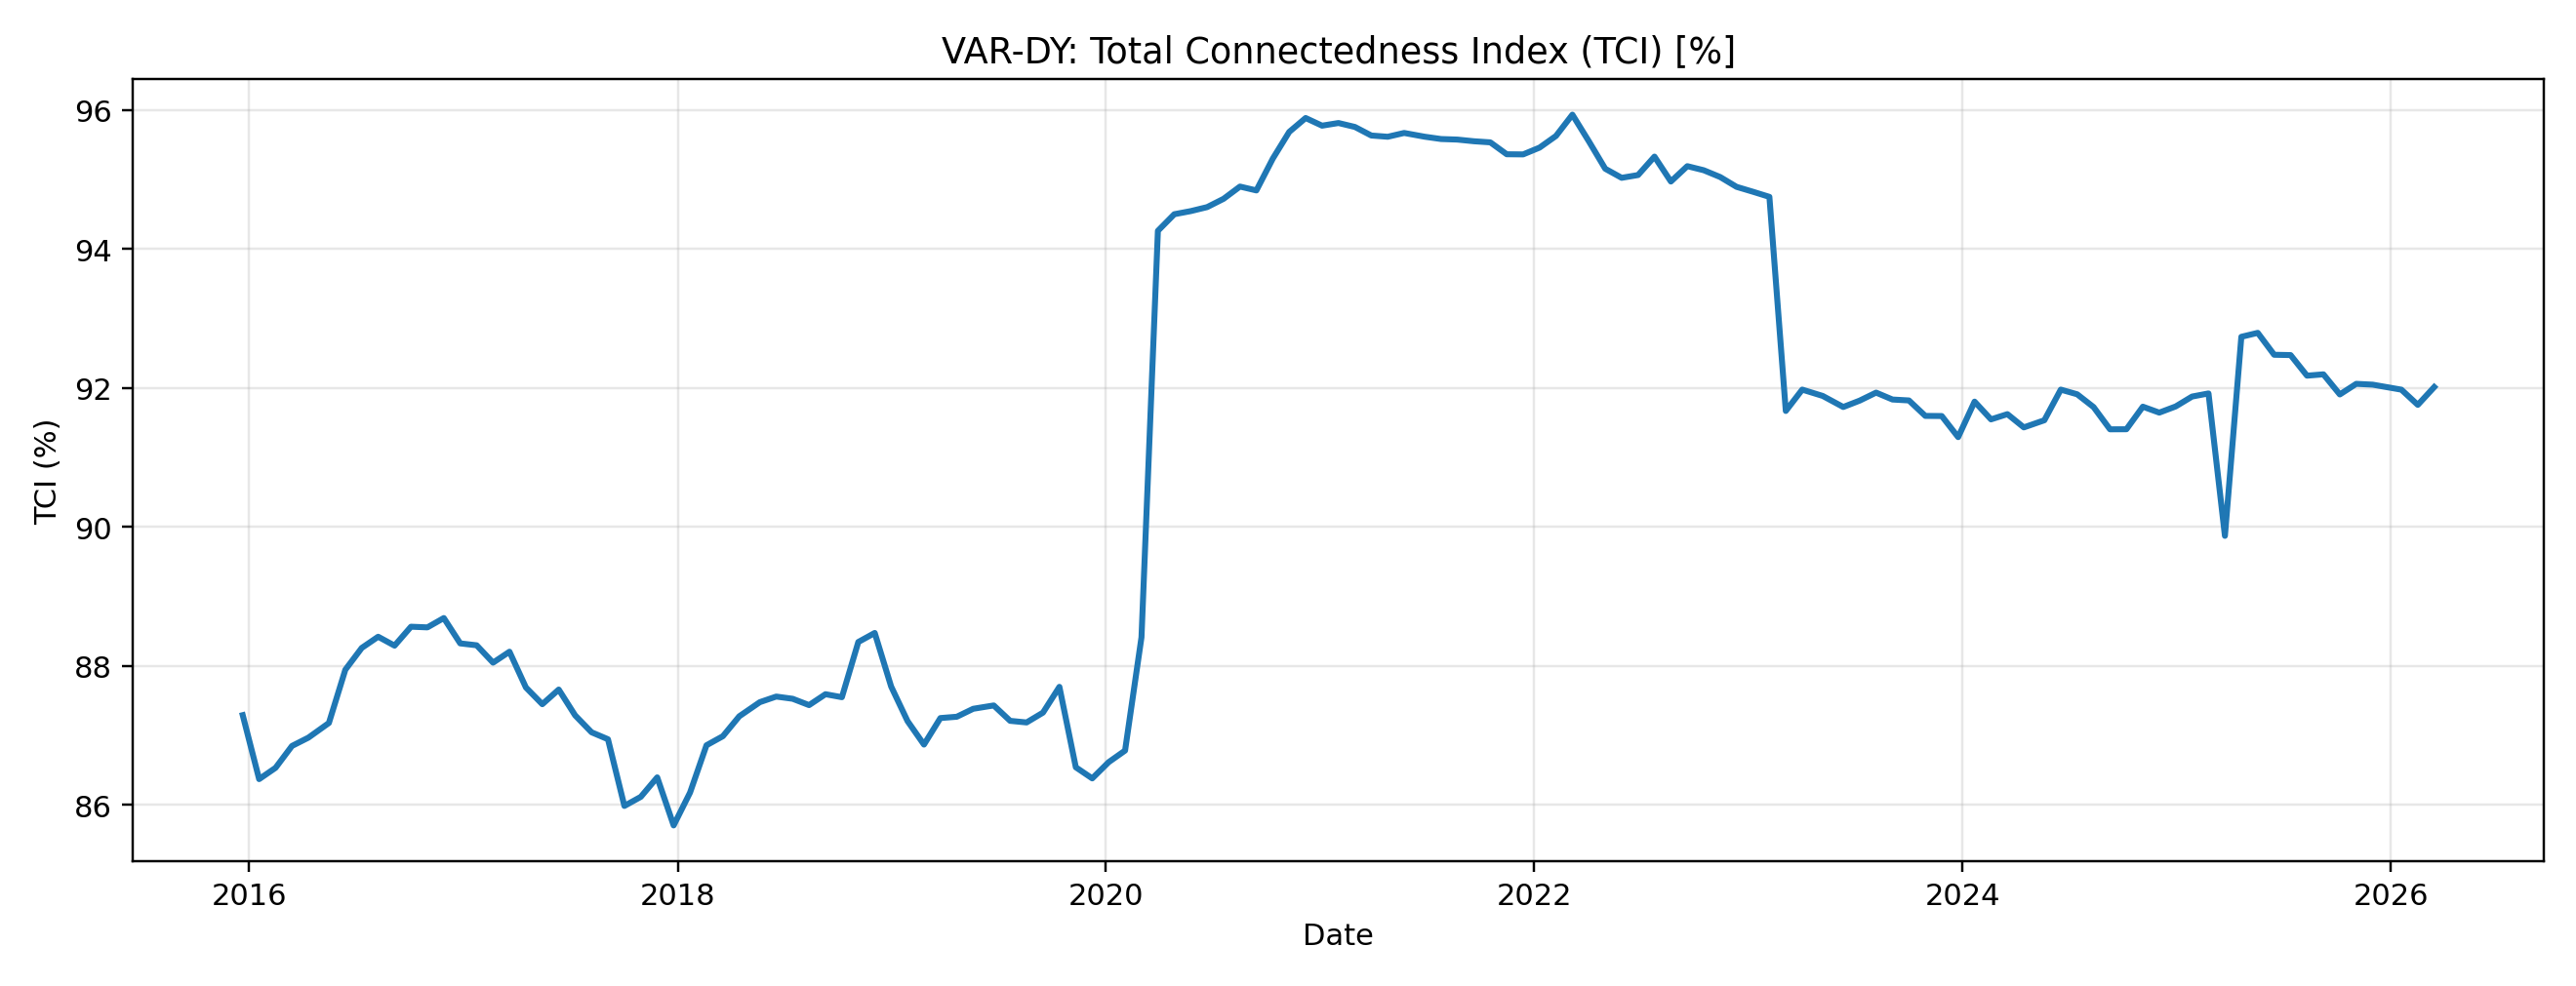
\includegraphics[width=\textwidth]{VAR_DY_tci_line.png}
  \caption{VAR--DY Total Connectedness Index (TCI) over time. The TCI measures the
  share of forecast error variance in standardized weekly log-returns explained by shocks
  to other institutions.}
  \label{fig:var_tci}
\end{figure}

Figure~\ref{fig:var_tci} displays the evolution of the Total Connectedness Index (TCI)
obtained from the rolling VAR--DY model. By construction, the TCI measures the average
share of forecast error variance in standardized weekly log-returns that is explained by
shocks to \emph{other} institutions (cross terms in the GFEVD), expressed in percentage
points.

Two main features stand out. First, even in tranquil periods the TCI remains high (around
the high 80s to low 90s), indicating that equity volatility for European financial
institutions is strongly interconnected: a large fraction of each institution's volatility
is attributable to system-wide shocks rather than idiosyncratic noise. Second, there is a
sharp, persistent jump in connectedness coinciding with the onset of the COVID--19 crisis.
Around early 2020 the TCI rises by several percentage points to levels close to $95\%$,
and stays elevated for an extended period before gradually normalizing. This pattern is
consistent with a common global shock that compresses risk premia and increases the
comovement of bank and insurer volatilities across Europe.

Post-crisis, the TCI declines from its peak but stabilizes at a level that remains above
most of the pre-2019 observations. This suggests that the COVID episode may have left a
lasting imprint on the structure of volatility spillovers, with European financials
remaining more tightly linked than before even once realized volatility itself recedes.

\paragraph{Formal structural break analysis.}

To move beyond visual inspection and formally integrate COVID-19 into the empirical
design, we apply the Bai--Perron (2003) multiple-break procedure and a targeted Chow
test to the TCI series (see Section~\ref{subsec:breaks}).

\begin{figure}[htbp]
  \centering
  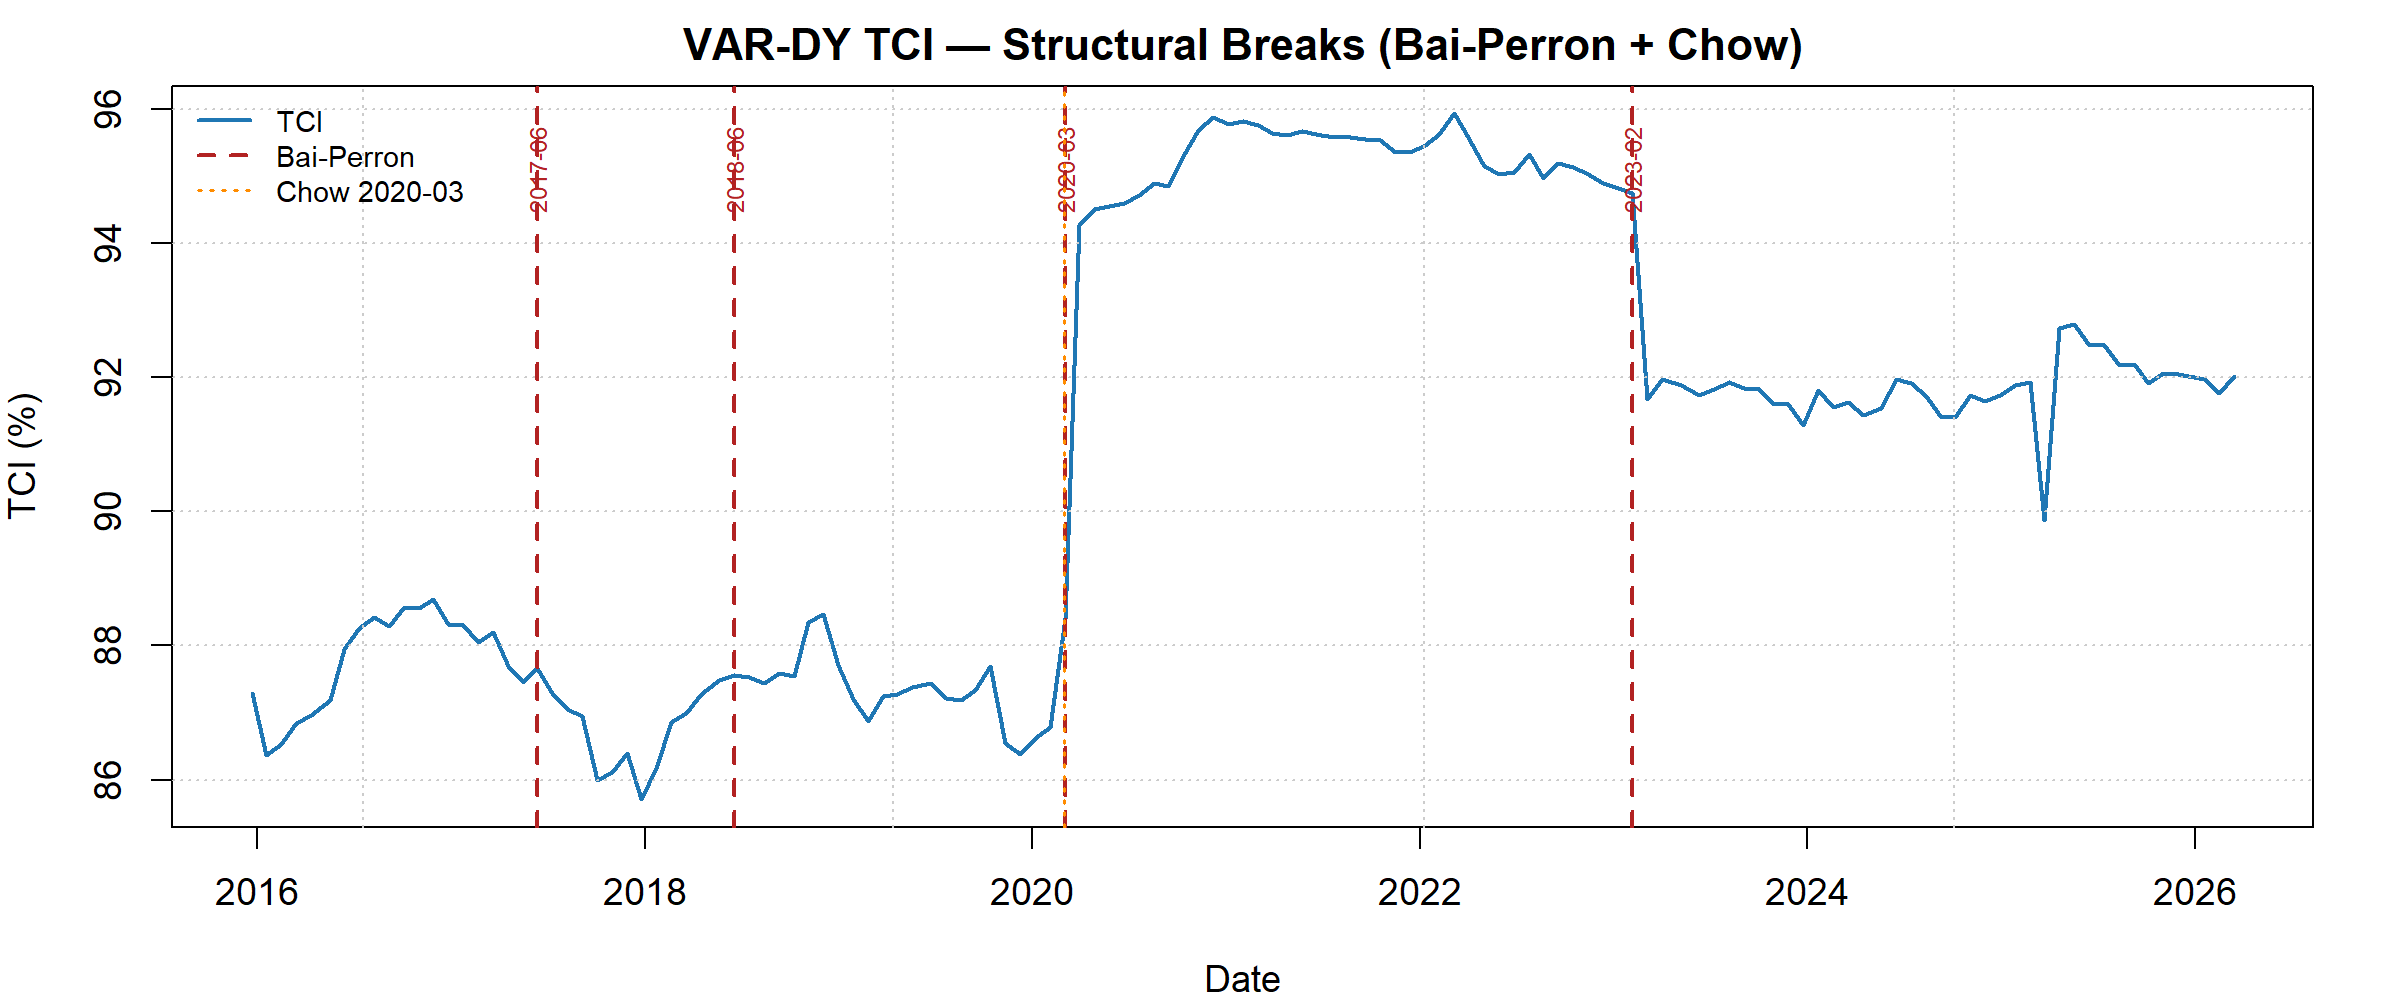
\includegraphics[width=\textwidth]{tci_with_breakpoints.png}
  \caption{VAR--DY Total Connectedness Index (TCI) with Bai--Perron structural break
  dates (vertical dashed lines) and 90\% confidence intervals (shaded bands). The Chow
  test at 2020-03-02 yields $F = 577.74$ ($p \approx 0$).}
  \label{fig:tci_breakpoints}
\end{figure}

Figure~\ref{fig:tci_breakpoints} displays the TCI series with the detected break dates
overlaid. The Bai--Perron procedure identifies four break dates: June 2017 [CI:
2017-02-20 to 2017-11-27], June 2018 [CI: 2017-10-02 to 2019-04-22], March 2020 [CI:
2020-02-03 to 2020-03-30], and February 2023 [CI: 2023-01-09 to 2023-03-06]. The Chow
test at 2020-03-02 yields $F = 577.74$ ($p \approx 0$), confirming a highly significant
structural shift coinciding with the COVID-19 onset. The 2020 break has by far the
tightest confidence interval (less than two months), reflecting the abruptness of the
pandemic shock relative to the more gradual transitions associated with the 2017--2018
breaks, which coincide with the unwinding of post-crisis ultra-loose monetary policy and
the early escalation of US--China trade tensions. The 2023 break corresponds to the
banking stress episode triggered by SVB/Credit Suisse failures. Post-break TCI
stabilises above pre-break norms, consistent with the structural ratchet
visible in Figure~\ref{fig:var_tci} and formally confirmed here.

\paragraph{Frequency decomposition of connectedness.}

The aggregate TCI series conflates volatility co-movement that operates at different
speeds. To distinguish transient contagion from durable structural integration, we apply
the frequency-domain decomposition of \citet{BarunikKrehlik2018} described in
Section~\ref{subsec:freq_conn}.

\begin{figure}[htbp]
  \centering
  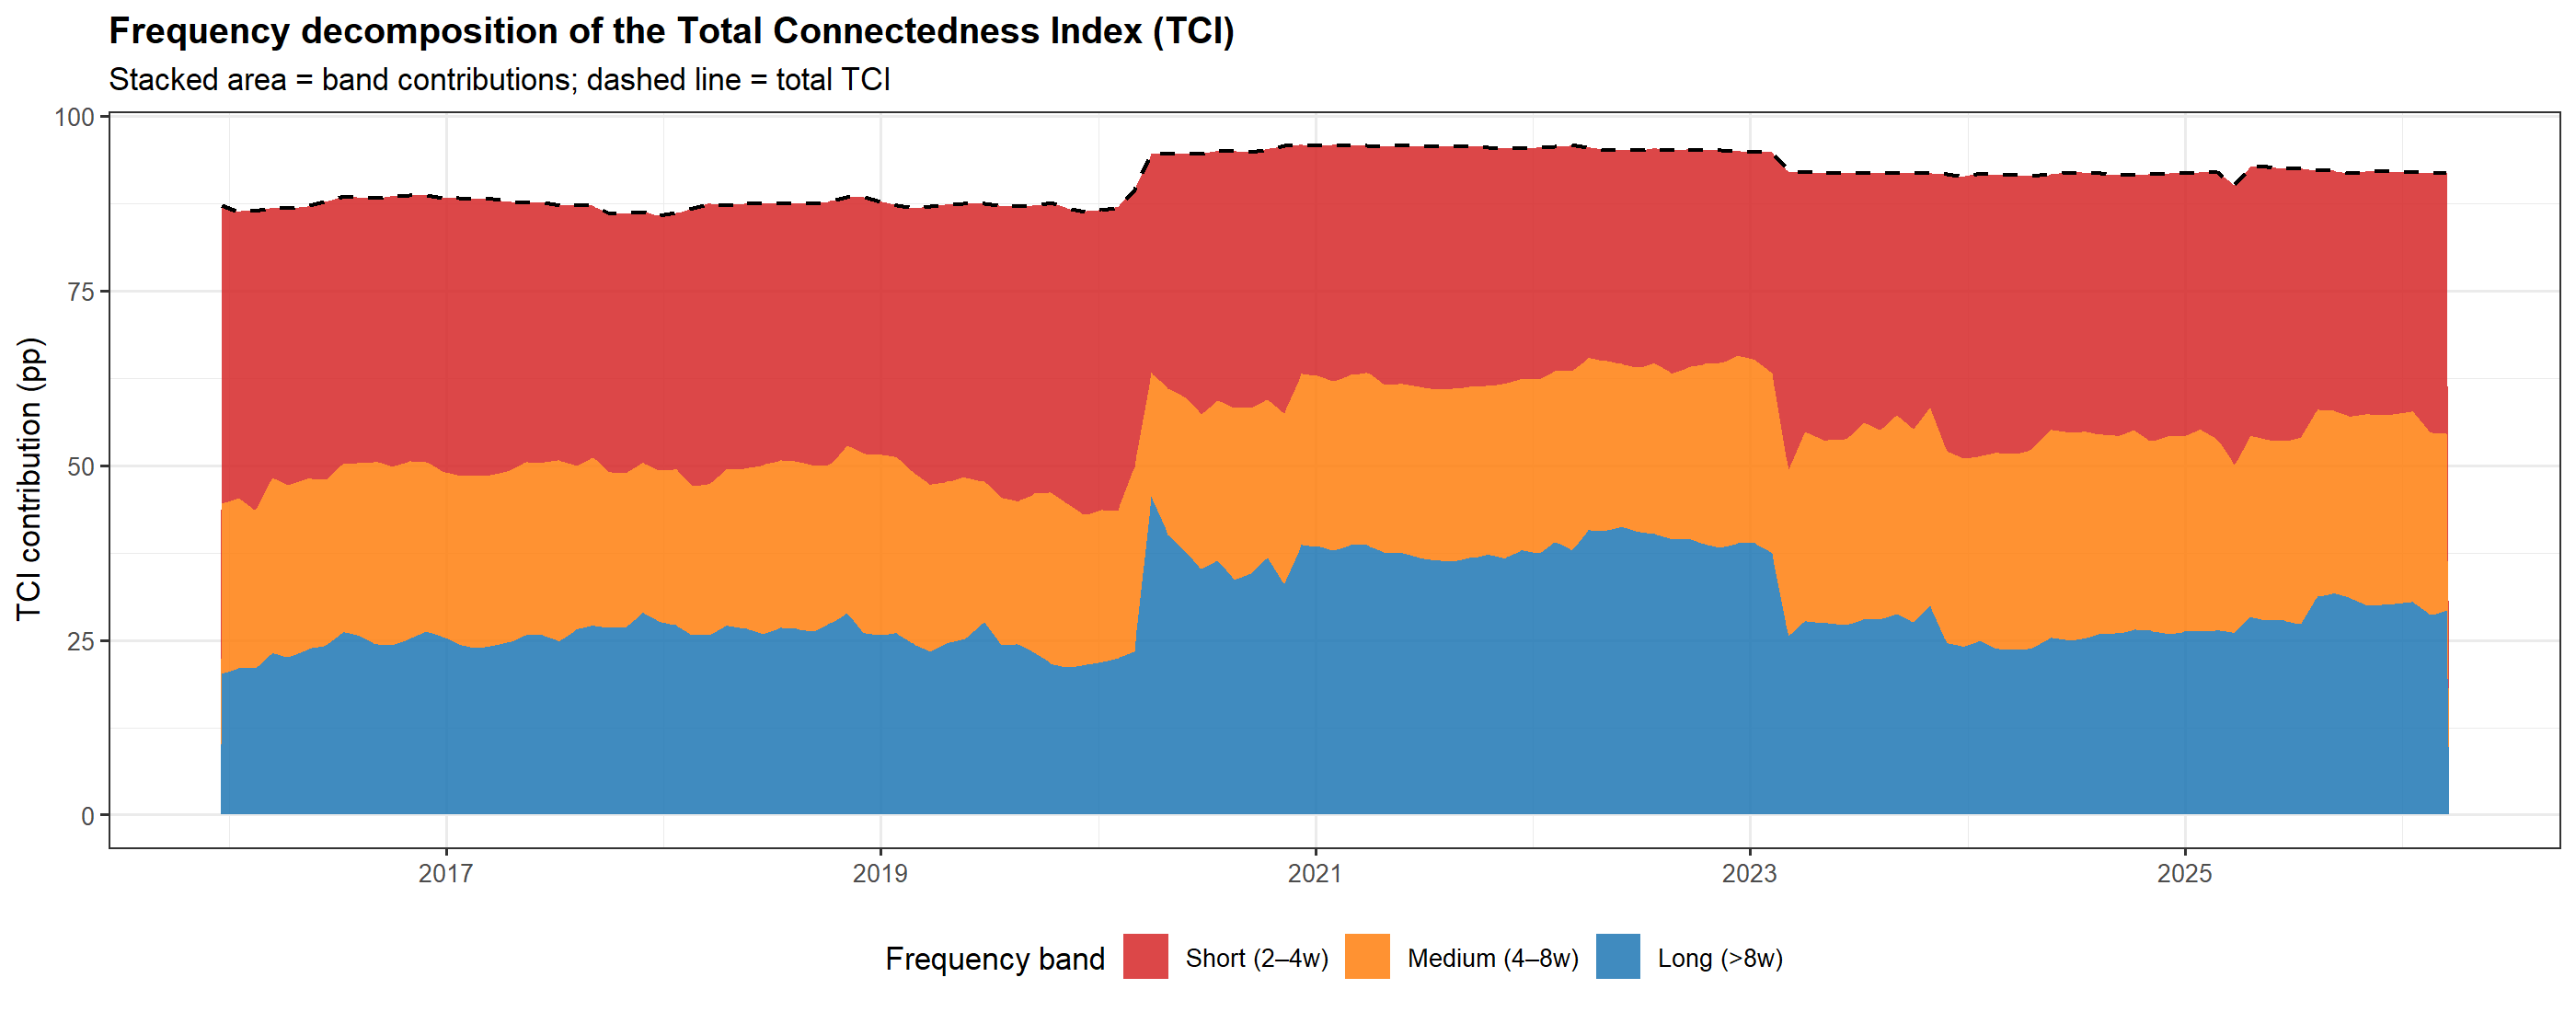
\includegraphics[width=\textwidth]{freq_tci_decomp.png}
  \caption{Frequency decomposition of the Total Connectedness Index. Stacked areas show
  the contributions of three bands to the aggregate TCI (dashed line): short-run
  (2--4 weeks, red), medium-run (4--8 weeks, orange), and long-run ($>$8 weeks, blue). On average, the three bands account for approximately 41\%, 27\%, and 32\% of
  the total TCI respectively.}
  \label{fig:freq_decomp}
\end{figure}

Figure~\ref{fig:freq_decomp} shows the stacked decomposition over the full sample. Three
findings stand out. First, in tranquil pre-COVID periods the short-run band dominates,
accounting for roughly 40\% of total connectedness, while medium- and long-run
contributions are broadly stable. This confirms that a large share of the structural
high-TCI baseline reflects fast market co-movement, not slow structural integration alone.

Second, and most strikingly, the COVID-19 shock triggers a sharp and \emph{persistent}
expansion of the \emph{long-run} band's share (from approximately 25\% to 45\%), while
the short-run share compresses. This pattern is counterintuitive from the perspective of
a purely transient panic: rather than spiking mainly in the short-run band and then
reverting, the pandemic durably rewired the slower structural linkages among European
financial institutions. The frequency decomposition thus provides direct evidence that the
post-COVID TCI ratchet documented in Section~\ref{subsec:rolling} reflects genuine
structural deepening, not a residual of short-term market disruption.

Third, the 2023 SVB/Credit Suisse episode is visible as a brief spike predominantly in
the short and medium bands, which then partially normalize, consistent with a
transient contagion episode that did not fundamentally restructure long-run dependencies.

\begin{figure}[htbp]
  \centering
  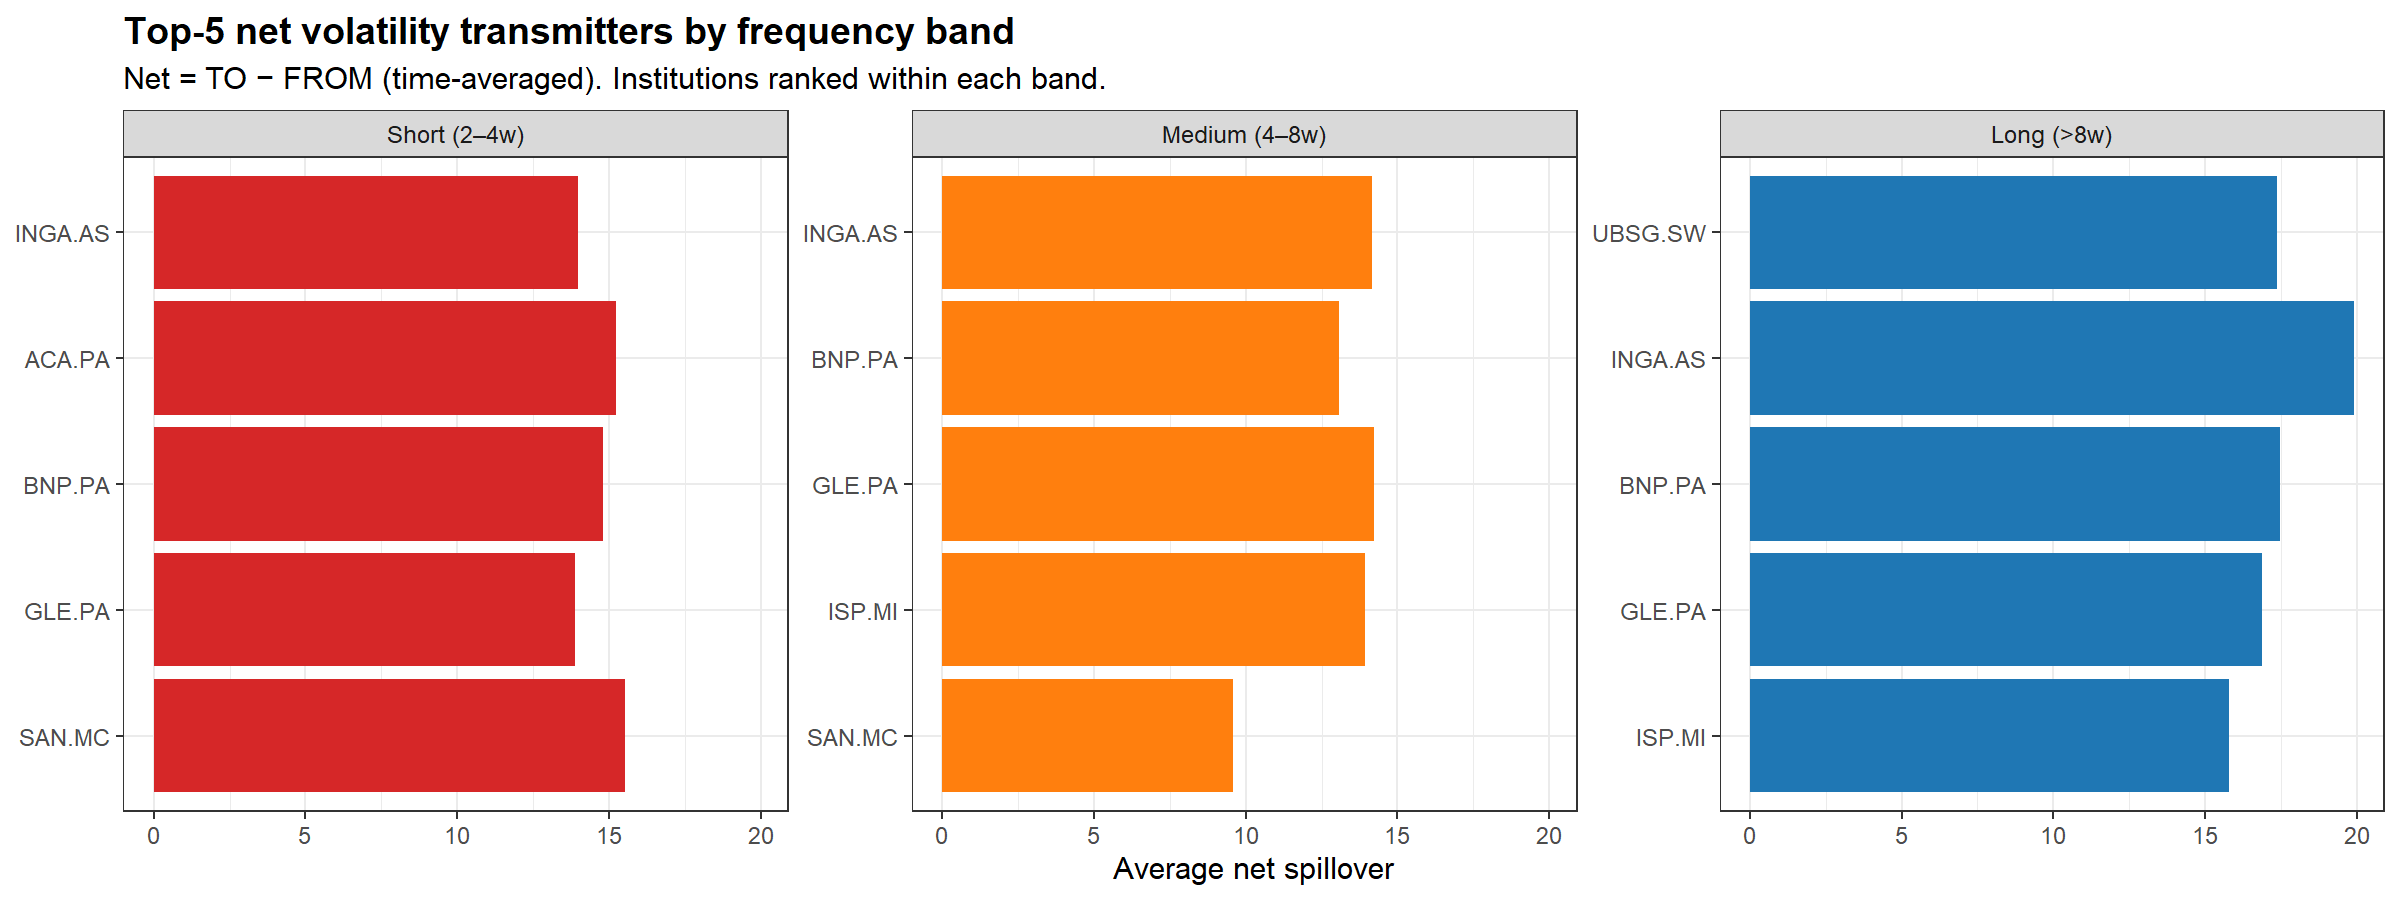
\includegraphics[width=\textwidth]{freq_top5_by_band.png}
  \caption{Top-5 net volatility transmitters by frequency band (time-averaged). Net =
  TO $-$ FROM. Institutions are ranked separately within each band.}
  \label{fig:freq_top5}
\end{figure}

Figure~\ref{fig:freq_top5} reveals that institutional roles differ markedly across
frequency bands. The French universal banks (BNP.PA, ACA.PA, GLE.PA) and Santander
(SAN.MC) dominate the short-run band, consistent with their heavy presence in
cross-border capital-market activities that transmit shocks rapidly. Notably, UBS
(UBSG.SW) appears as the top long-run transmitter but is absent from the short-run
top-5 entirely, reflecting its role as a structurally integrated wealth-management and
investment hub with long-horizon balance-sheet exposures rather than a channel for fast
contagion. This institution-level frequency heterogeneity cannot be detected from the
aggregate time-domain net spillovers alone, and has direct implications for
macroprudential surveillance: short-run and long-run systemic risk hubs may warrant
distinct supervisory treatment.

% ---------------------------------------------------------------
\subsection{Directional connectedness: major receivers and emitters}
% ---------------------------------------------------------------

To understand which institutions drive these system-wide dynamics, we analyze
cross-sectional rankings of directional connectedness. For each institution $i$, we
compute time-averaged measures of volatility received \emph{from} the system,
\[
  \overline{C}_{i \leftarrow \bullet}
  = \frac{1}{W^\ast} \sum_{w=1}^{W^\ast} C_{i \leftarrow \bullet, w},
\]
and volatility transmitted \emph{to} the system,
\[
  \overline{C}_{i \rightarrow \bullet}
  = \frac{1}{W^\ast} \sum_{w=1}^{W^\ast} C_{i \rightarrow \bullet, w},
\]
together with the associated net measure
\[
  \overline{C}_i^{\text{net}}
  = \overline{C}_{i \rightarrow \bullet} - \overline{C}_{i \leftarrow \bullet}.
\]

\begin{figure}[htbp]
  \centering
  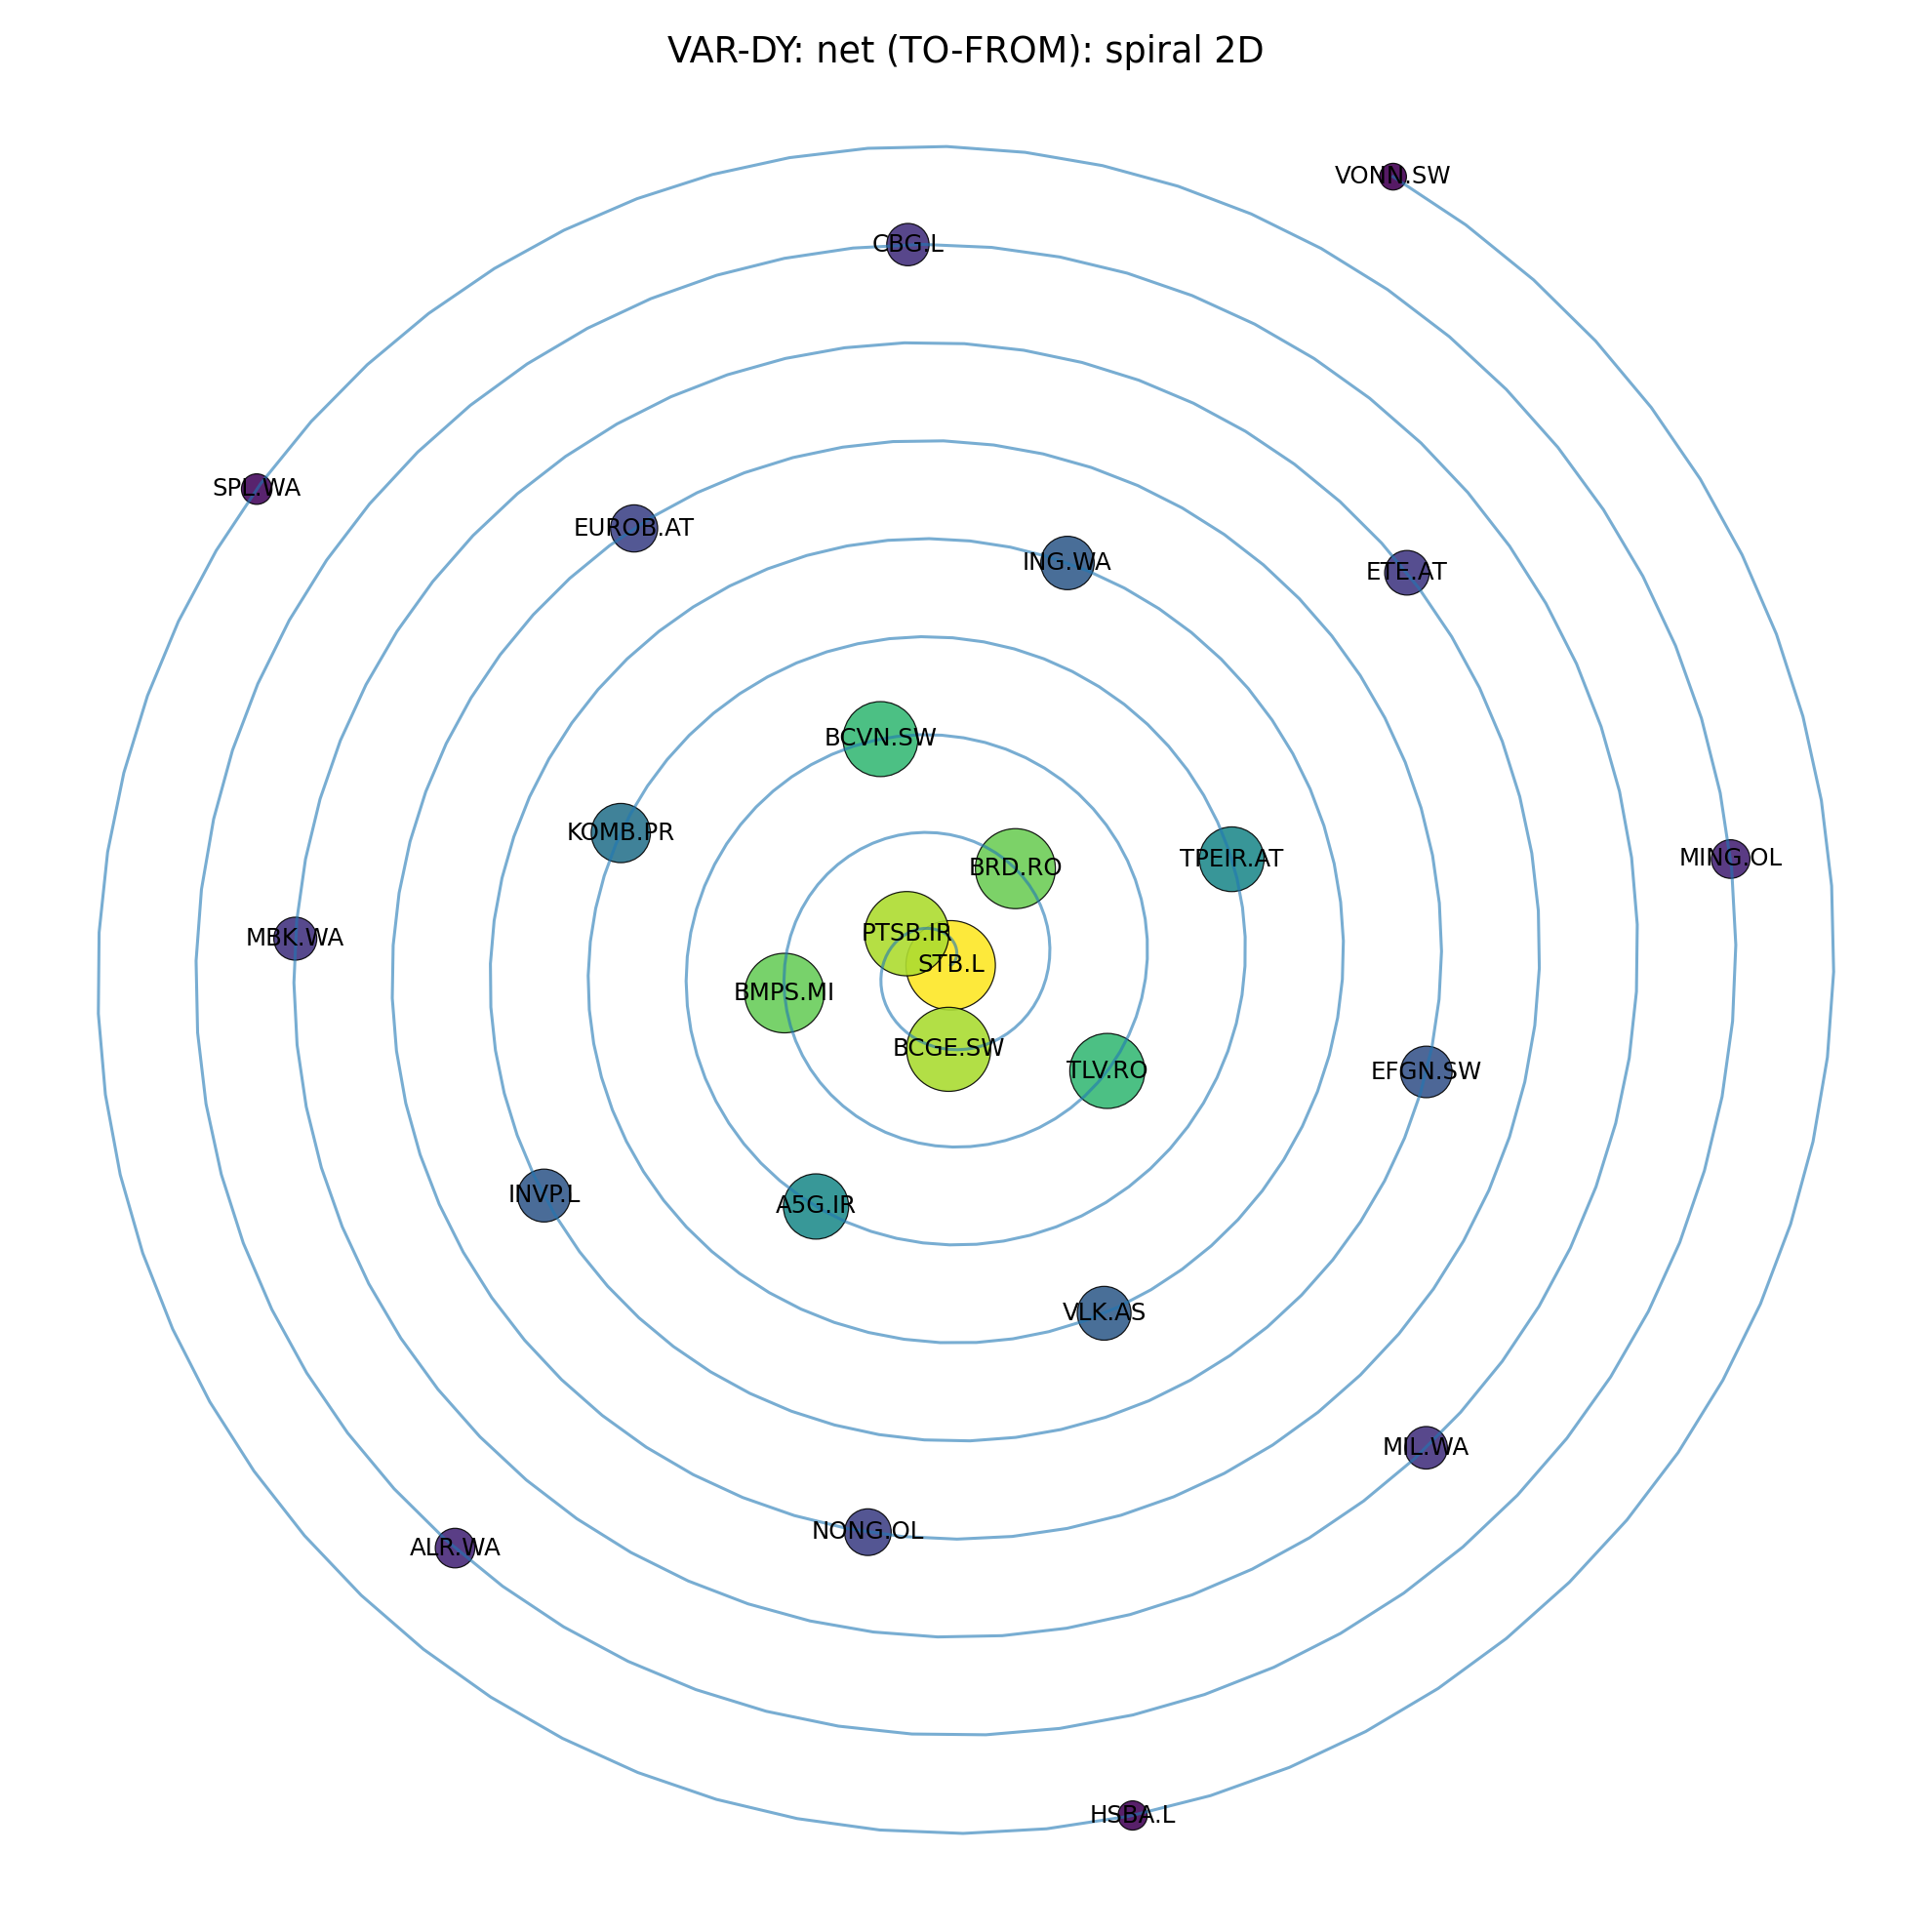
\includegraphics[width=\textwidth]{VAR_DY_helix_NET_spiral.png}
  \caption{Net spillovers (TO$-$FROM) in VAR--DY: 2D spiral representation. Institutions
  with the largest positive net measures (net transmitters) cluster near the centre; net
  receivers are pushed outward. Detailed FROM, TO, and helix representations are provided
  in Appendix~\ref{app:additional}.}
  \label{fig:var_net_spiral}
\end{figure}

Cross-sectional directional rankings show that a small core of large universal banks acts
simultaneously as top receivers and top emitters (see Appendix~\ref{app:additional} for
FROM and TO spiral plots). Major French, Dutch, Spanish, and Swiss institutions
(BNP Paribas, Société Générale, ING, Santander, UBS) appear among the top receivers,
while large cross-border banks with significant capital-market activities dominate the
emitter ranking. To isolate pure spillover direction, Figure~\ref{fig:var_net_spiral}
ranks institutions by net connectedness $\overline{C}_i^{\text{net}}$.

The net ranking highlights a group of banks from peripheral or smaller European markets
that are persistent exporters of volatility to the rest of the system. Conversely,
several large Western European institutions emerge as structural net receivers: they
absorb more volatility from others than they transmit on average. This asymmetry in net
spillovers has direct implications for systemic-risk monitoring: net transmitters are
natural candidates for ``outward'' stress channels, whereas net receivers are more exposed
to contagion from shocks originating elsewhere.

Overall, the VAR--DY results suggest that (i)~European financial equities form a tightly
interconnected volatility network, especially during global crises; (ii)~a relatively
small set of large institutions sits at the core of the network as both major receivers
and emitters; and (iii)~there is a non-trivial subset of banks that act as structural net
transmitters or net receivers of volatility. The persistent dominance of large universal
banks (BNP Paribas, Société Générale, ING, Santander, UBS) as central nodes is
consistent with their extensive cross-border balance sheet exposures, their role in
wholesale funding markets, and the fact that their equity prices aggregate information
from multiple regulatory and sovereign environments simultaneously. Peripheral-market
institutions, by contrast, tend to act as net transmitters partly because their smaller
size makes them more sensitive to system-wide shocks that originate in core markets,
and partly because their local sovereign risks generate domestic spillovers that
reverberate into the wider European system. These rankings will be formally compared to
centrality measures from correlation-based and MST networks in Section~\ref{subsec:centrality}.

% ---------------------------------------------------------------
\subsection{DCC--GARCH dependence and correlation networks}
% ---------------------------------------------------------------

We now turn to the covariance-based benchmark provided by the DCC--GARCH model described
in Section~\ref{subsec:dcc}. For the full sample, we estimate univariate GARCH(1,1)
models for all returns, extract standardized residuals, and fit a DCC specification with
parameters $(a,b)$ constrained so that $a + b < 1$. This yields a sequence of
conditional correlation matrices $\{R_t\}$ that can be aligned with the VAR--DY rolling
windows, allowing a direct comparison between connectedness and correlation-based
measures.

\paragraph{Mean absolute correlation over time.}

For each date $t$, we summarize the cross-sectional dependence by the average absolute
pairwise correlation
\begin{equation}
  \overline{\rho}_t
  = \frac{2}{N(N-1)} \sum_{1 \le i < j \le N} \big|\rho_{ij,t}\big|,
\end{equation}
computed from the DCC correlation matrices $R_t$.
Figure~\ref{fig:dcc_meanabs} plots the resulting time series of $\overline{\rho}_t$.

\begin{figure}[htbp]
  \centering
  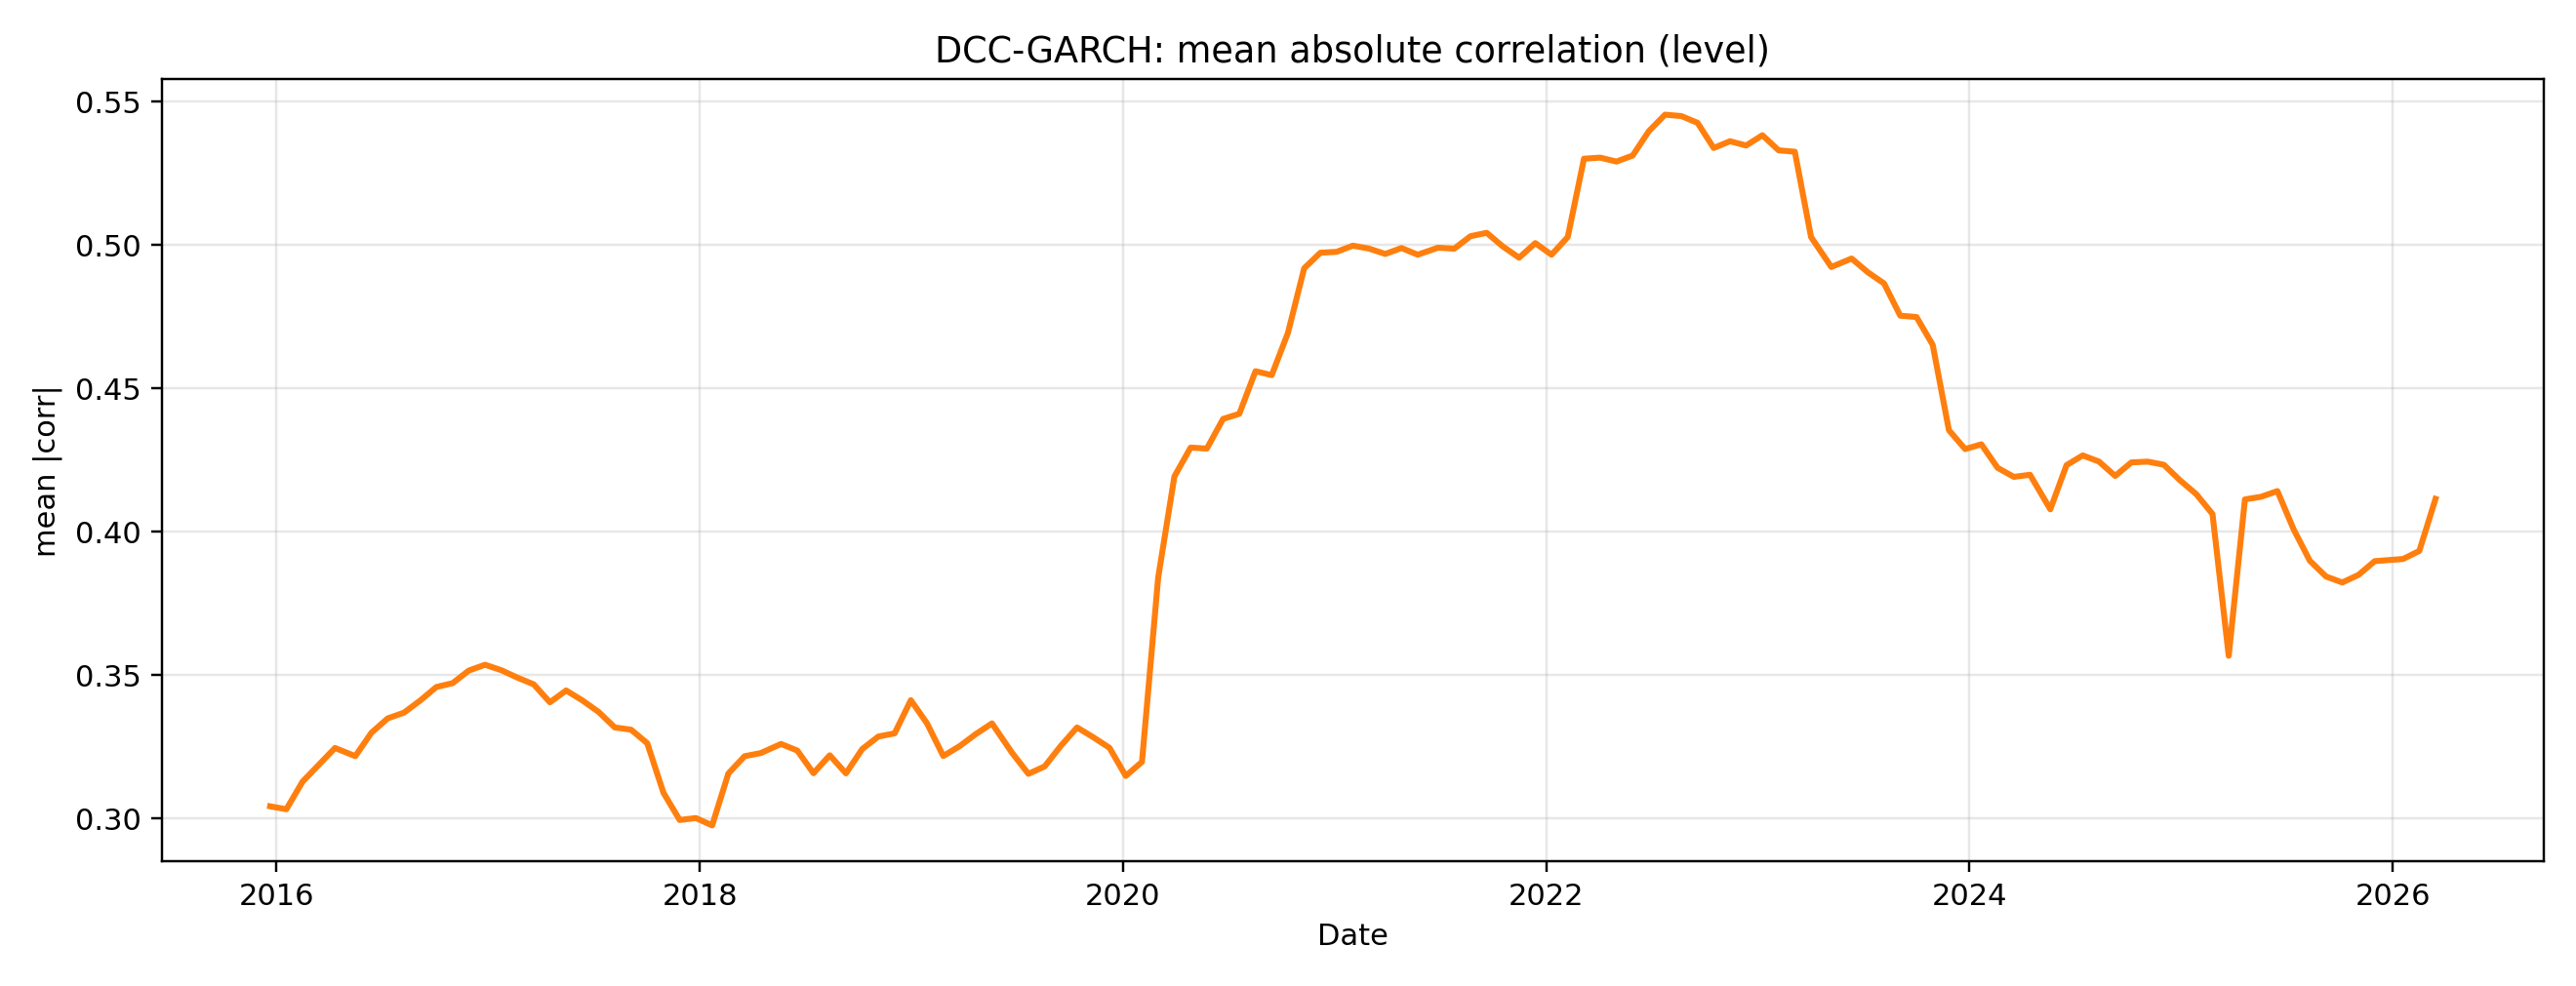
\includegraphics[width=\textwidth]{DCC_mean_abs_corr_line.png}
  \caption{DCC--GARCH: time series of the mean absolute pairwise correlation
  $\overline{\rho}_t$ across European financial institutions.}
  \label{fig:dcc_meanabs}
\end{figure}

Two patterns mirror the VAR--DY results. First, even in calm periods the mean correlation
stays around $0.30$--$0.35$, confirming that European financial equities are structurally
interdependent. Second, there is a pronounced jump in $\overline{\rho}_t$ at the onset
of the COVID--19 crisis, with average correlations moving above $0.50$ and remaining
elevated for several quarters before gradually declining. The timing of this spike closely
matches the increase in the VAR-based TCI, indicating that both approaches capture the
same surge in systemic comovement during the pandemic. Post-crisis, the mean correlation
falls but stabilizes at a level that is still higher than most pre-2019 observations,
suggesting a persistent tightening of cross-institution linkages.

The cross-sectional correlation heatmap and eigenvector centrality time series are provided in Appendix~\ref{app:additional}. Top DCC-central institutions (typically above $0.85$ eigenvector centrality) largely overlap with the VAR--DY core, confirming that econometric connectedness and correlation-based centrality point to the same set of systemically important institutions.

Overall, the DCC results corroborate the VAR--DY evidence. Both frameworks indicate that
(i)~European financial institutions form a highly interconnected system even in tranquil
times; (ii)~systemic comovement rises sharply during global crises such as COVID--19; and
(iii)~a relatively small set of large cross-border banks occupies the core of the
network. We now confront these findings with the joint behaviour of the VAR--DY TCI and
the mean DCC correlation, and with cluster-level connectedness patterns.

% ---------------------------------------------------------------
\subsection{Comparing VAR--DY connectedness and DCC
correlations}\label{subsec:compare_dy_dcc}
% ---------------------------------------------------------------

To relate the econometric notion of connectedness to a more standard, correlation-based
view of dependence, we compare the VAR--DY Total Connectedness Index to the mean absolute
DCC correlations. For each VAR window $w$ we compute the system-wide $\mathrm{TCI}_w$
and, on the same set of dates, the cross-sectional average of the absolute DCC
correlations (Section~\ref{subsec:dcc}), expressed in percentage points.

\begin{figure}[t!]
  \centering
  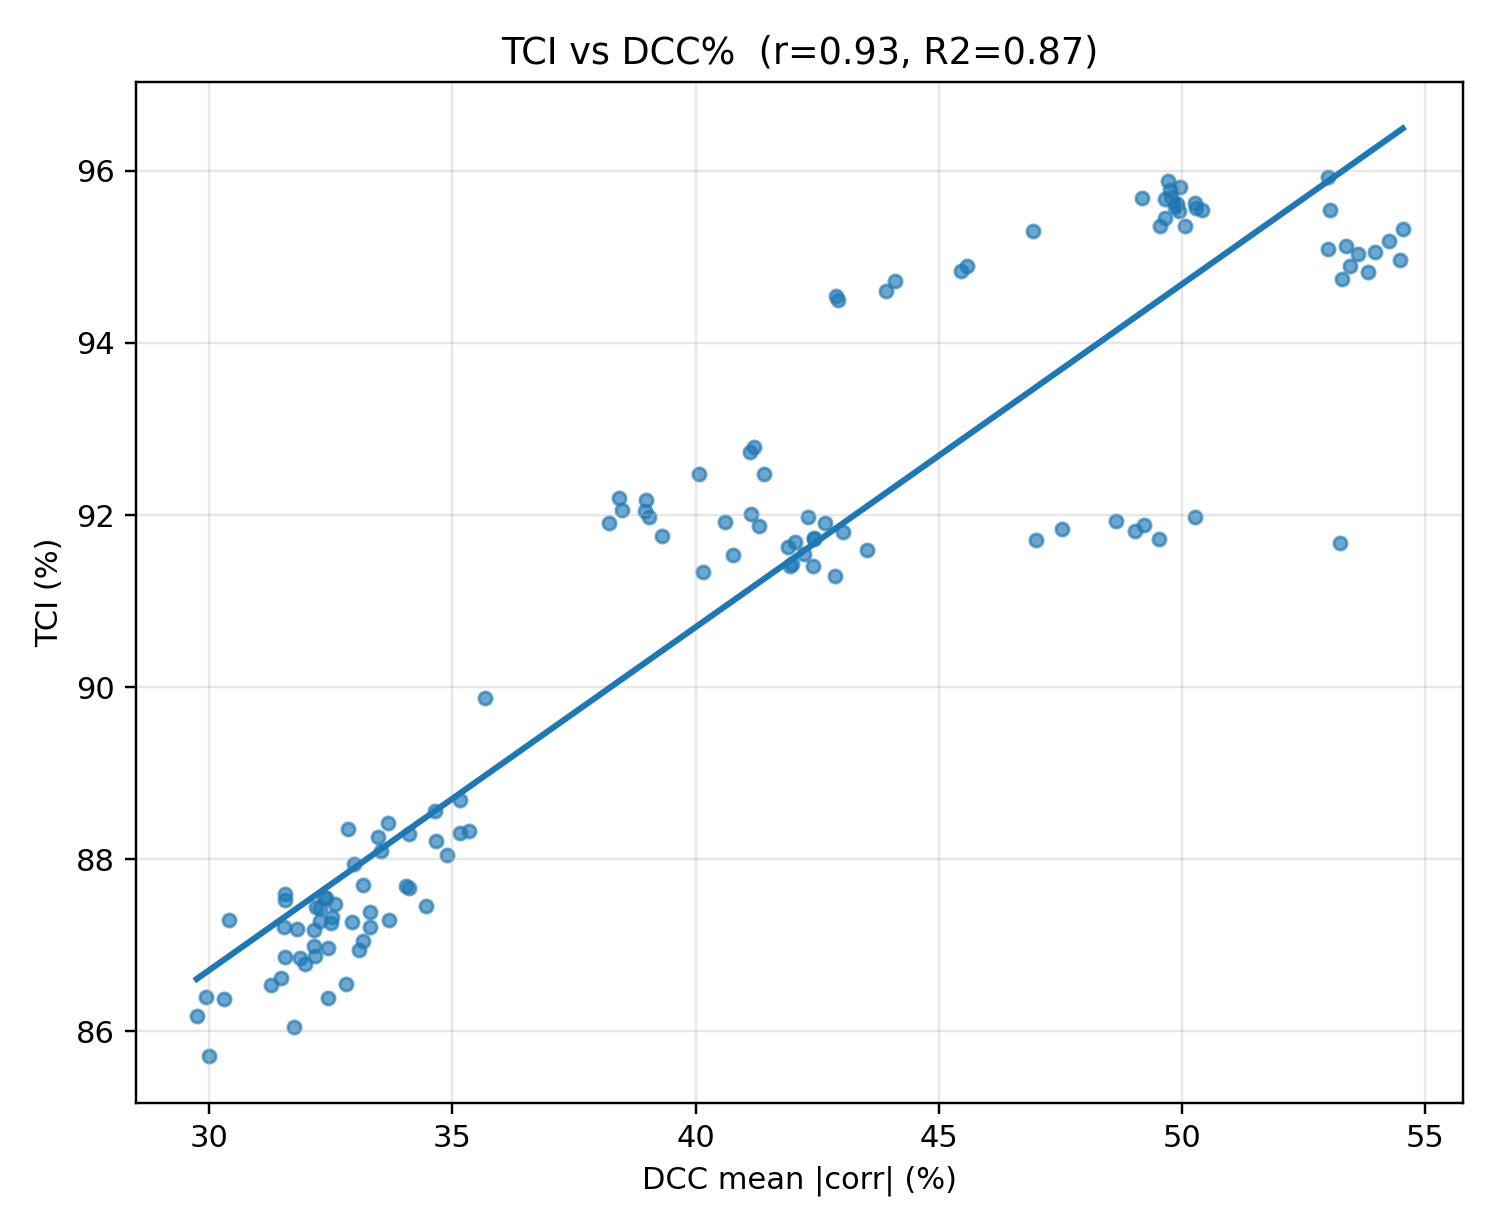
\includegraphics[width=0.7\textwidth]{DY_DCC_scatter_reg.png}
  \caption{Scatter plot of TCI versus mean absolute DCC correlation (both in percent)
  with fitted regression line. Pearson $r \approx 0.94$, $R^2 \approx 0.88$.
  Time-series levels, rolling correlation, and cross-correlation plots are in
  Appendix~\ref{app:additional}.}
  \label{fig:dy_dcc_scatter}
\end{figure}

Figure~\ref{fig:dy_dcc_scatter} plots $\mathrm{TCI}_w$ against mean $\mathrm{DCC}_w$
across all windows. Points lie close to the fitted OLS line ($\widehat{\mathrm{TCI}} =
75.11 + 0.39\,\mathrm{DCC}$), with a Pearson correlation of $0.94$ and $R^2 \simeq
0.88$. The cross-correlation function (Appendix~\ref{app:additional}) peaks at lag $-1$,
meaning that changes in DCC-based correlations marginally precede changes in
variance-decomposition connectedness. Overall, both measures provide quantitatively
consistent pictures of systemic comovement, validating the VAR--DY framework against a
simpler, model-free benchmark. We now synthesize the full set of rolling estimates by
applying $k$-means clustering to GFEVD feature vectors, identifying the distinct
connectedness regimes that emerge from the data.

% ---------------------------------------------------------------
\subsection{Connectedness regimes}\label{subsec:regime_results}
% ---------------------------------------------------------------

Applying $k$-means to the five-feature GFEVD summary vectors described in
Section~\ref{subsec:regimes}, the silhouette criterion selects $K^{*} = 2$ regimes
(mean silhouette $= 0.54$, substantially above all higher-$K$ alternatives;
$K$-selection diagnostics in Appendix~\ref{app:additional}). The two-regime structure is
therefore not an arbitrary choice but emerges directly from the data.

\begin{figure}[htbp]
  \centering
  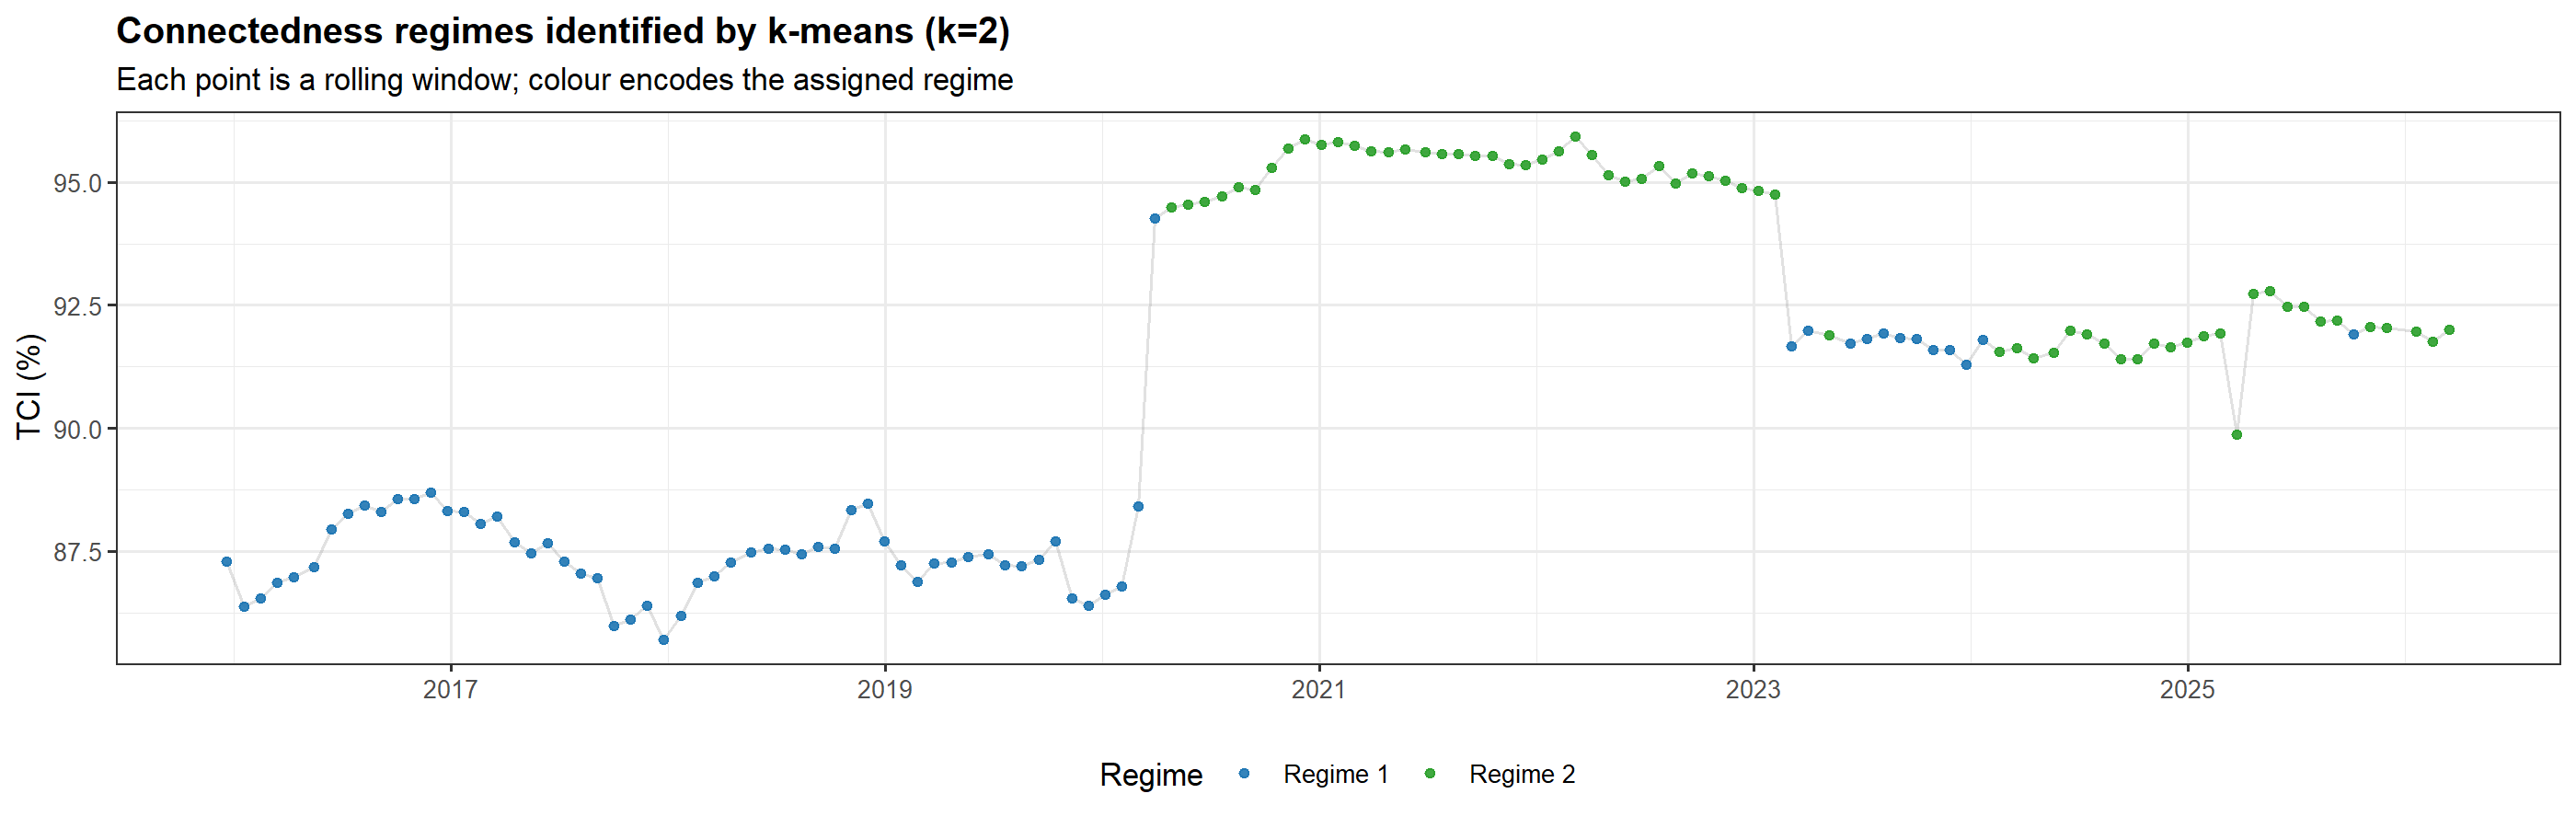
\includegraphics[width=\textwidth]{regime_timeline.png}
  \caption{Connectedness regime assignment over time. Each point represents one rolling
  window; colour encodes the assigned regime. Regime~1 (low connectedness, TCI $\approx
  88\%$) corresponds to calm market periods; Regime~2 (high connectedness, TCI $\approx
  94\%$) corresponds to systemic-stress episodes, most prominently the COVID-19 shock
  and its aftermath.}
  \label{fig:regime_timeline}
\end{figure}

Figure~\ref{fig:regime_timeline} shows regime assignments over time.
Table~\ref{tab:regime_profiles} summarises the mean feature profiles of each regime.

\begin{table}[htbp]
  \centering
  \caption{Mean feature profiles by connectedness regime ($K^{*} = 2$, $n=132$ windows).}
  \label{tab:regime_profiles}
  \begin{tabular}{lrrrrrr}
  \hline
  Regime & Windows & TCI (\%) & $\sigma(\text{NET})$ & max NET &
           Top-5 TO share & Skew(NET) \\
  \hline
  1 (Calm)   & 68 & 88.2 & 28.4 & 61.6 & 0.133 & $+0.19$ \\
  2 (Crisis) & 64 & 93.8 & 26.2 & 50.2 & 0.117 & $-0.52$ \\
  \hline
  \end{tabular}
\end{table}

Three features of the regime profiles stand out. First, the TCI gap between regimes is
approximately 5.6 percentage points (88.2\% vs.\ 93.8\%), confirming that the two
regimes capture meaningfully different levels of systemic connectedness rather than noise.
Second, the crisis regime (Regime 2) is characterized by \emph{lower} cross-sectional
dispersion ($\sigma(\mathrm{NET})$) and a lower maximum net spillover despite higher
aggregate connectedness, a hallmark of network homogenization under stress: shocks
become more uniformly distributed and the dominance of any single transmitter diminishes
relative to the system as a whole. Third, the negative skewness of Regime 2 ($-0.52$
vs.\ $+0.19$) indicates that during crises, the net-spillover distribution tilts toward
more institutions becoming net receivers while a smaller number become strong net
transmitters. These structural shifts are invisible to aggregate TCI analysis alone, and
their cross-sectional implications are examined in the next subsection.

% ---------------------------------------------------------------
\subsection{Cross-method centrality alignment}\label{subsec:centrality}
% ---------------------------------------------------------------

A central methodological question is whether institutions identified as structurally
important by the VAR--DY framework are also central in purely statistical
correlation-based and network approaches. If both model-based and model-free methods
point to the same set of systemic hubs, this provides strong cross-method robustness
for the risk rankings; if they diverge, the choice of methodology would be consequential
for macroprudential surveillance.

To place all three methods on a common footing, we compare each institution's
time-averaged VAR--DY \emph{TO} strength $\bar\theta_i^{\mathrm{TO}}$ against two
analogous strength measures computed from purely statistical networks: the correlation
strength $\sum_{j\neq i}|\hat\rho_{ij}|$ (full pairwise matrix) and the MST weighted
degree $\sum_{(i,j)\in\mathcal{T}}|\hat\rho_{ij}|$ (sum of absolute correlations on
incident spanning-tree edges). Figure~\ref{fig:strength_scatter} displays both
comparisons.

The Spearman rank correlation between VAR--DY TO strength and correlation strength is
$\rho = 0.97$ ($p \approx 0$, $n = 63$), indicating near-perfect alignment across the full
institutional cross-section. Even a model-free, statistically simple correlation network
recovers essentially the same systemic risk hierarchy as the more sophisticated
variance-decomposition framework. The alignment with MST weighted degree is $\rho = 0.70$
($p \approx 0$, $n = 63$), indicating strong and statistically highly significant
agreement. Using a weighted degree rather than simple edge count brings the MST ranking
closer to the econometric one: the residual gap reflects the additional topological
constraints imposed by spanning-tree extraction, which retains only the $N-1$ minimum-distance
edges and therefore discards some weaker but non-negligible correlation links.

\begin{figure}[htbp]
  \centering
  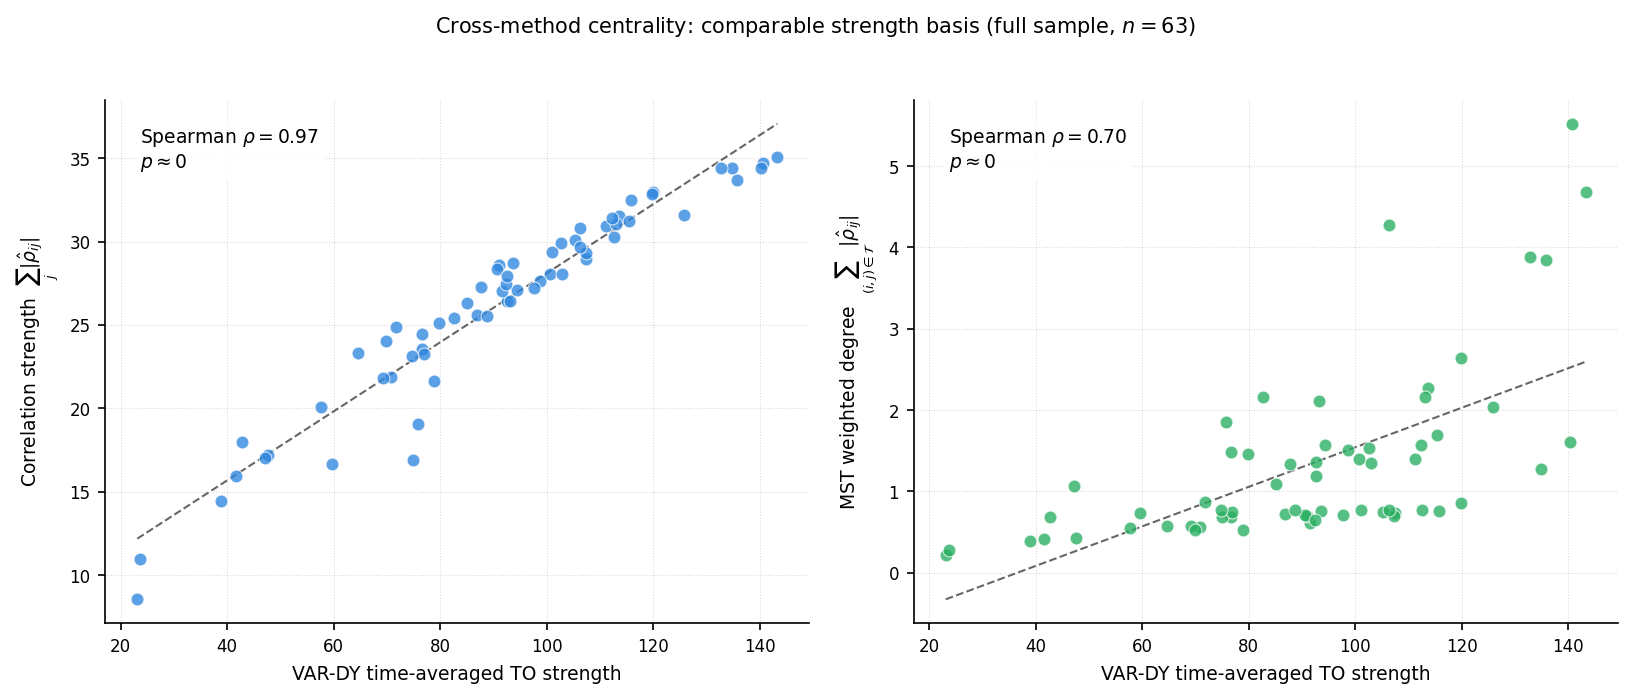
\includegraphics[width=\textwidth]{centrality_strength_comparison.png}
  \caption{Cross-method centrality on a comparable strength basis (full sample, $n=63$).
  \emph{Left}: VAR--DY time-averaged TO strength ($\bar\theta_i^{\mathrm{TO}}$) versus
  correlation strength $\sum_{j\neq i}|\hat\rho_{ij}|$; Spearman $\rho = 0.97$, $p \approx 0$.
  \emph{Right}: VAR--DY TO strength versus MST weighted degree $\sum_{(i,j)\in\mathcal{T}}|\hat\rho_{ij}|$;
  Spearman $\rho = 0.70$, $p \approx 0$.
  Dashed lines are OLS trend lines.}
  \label{fig:strength_scatter}
\end{figure}

These results validate the claim that institutions occupying central positions in the
econometric spillover network are also hubs in correlation-based networks, providing
strong cross-method robustness for the systemic risk rankings reported above.

\paragraph{Institutional stability across methods and regimes.}

Decomposing this alignment to the institutional level (Appendix~\ref{app:additional}),
BNP Paribas (BNP.PA) appears among the top-5 by strength centrality across all nine
method--period cells (three methods $\times$ three sub-periods), and Santander (SAN.MC),
Société Générale (GLE.PA), Crédit Agricole (ACA.PA), and ING (INGA.AS) feature
consistently in the majority. The core group of systemically important institutions is
therefore not an artefact of a particular modelling choice or of a specific market
episode; it is a structural feature of the European financial system that survives changes
in estimation methodology, risk measure, and economic regime. Detailed rank heatmaps
across the top-10 institutions and both strength and betweenness centrality are provided
in Appendix~\ref{app:centrality_heatmaps}.

% ---------------------------------------------------------------
\subsection{Cluster-level connectedness by country}\label{subsec:tci_clusters}
% ---------------------------------------------------------------

Within-country TCI time series for all 18 countries are shown in Appendix~\ref{app:additional}. All countries exhibit very high within-cluster connectedness (typically above $90\%$), confirming that equity volatility is strongly driven by common domestic shocks. However, there is substantial cross-country heterogeneity: core Eurozone markets (DE, FR, NL) display smooth but persistently high TCI paths, whereas peripheral markets (PL, NO, UK) feature more pronounced swings. The COVID--19 episode either amplifies or partially offsets domestic co-movement depending on local balance-sheet structures and policy responses, providing a natural guide for cross-country diversification.

\begin{figure}[t!]
  \centering
  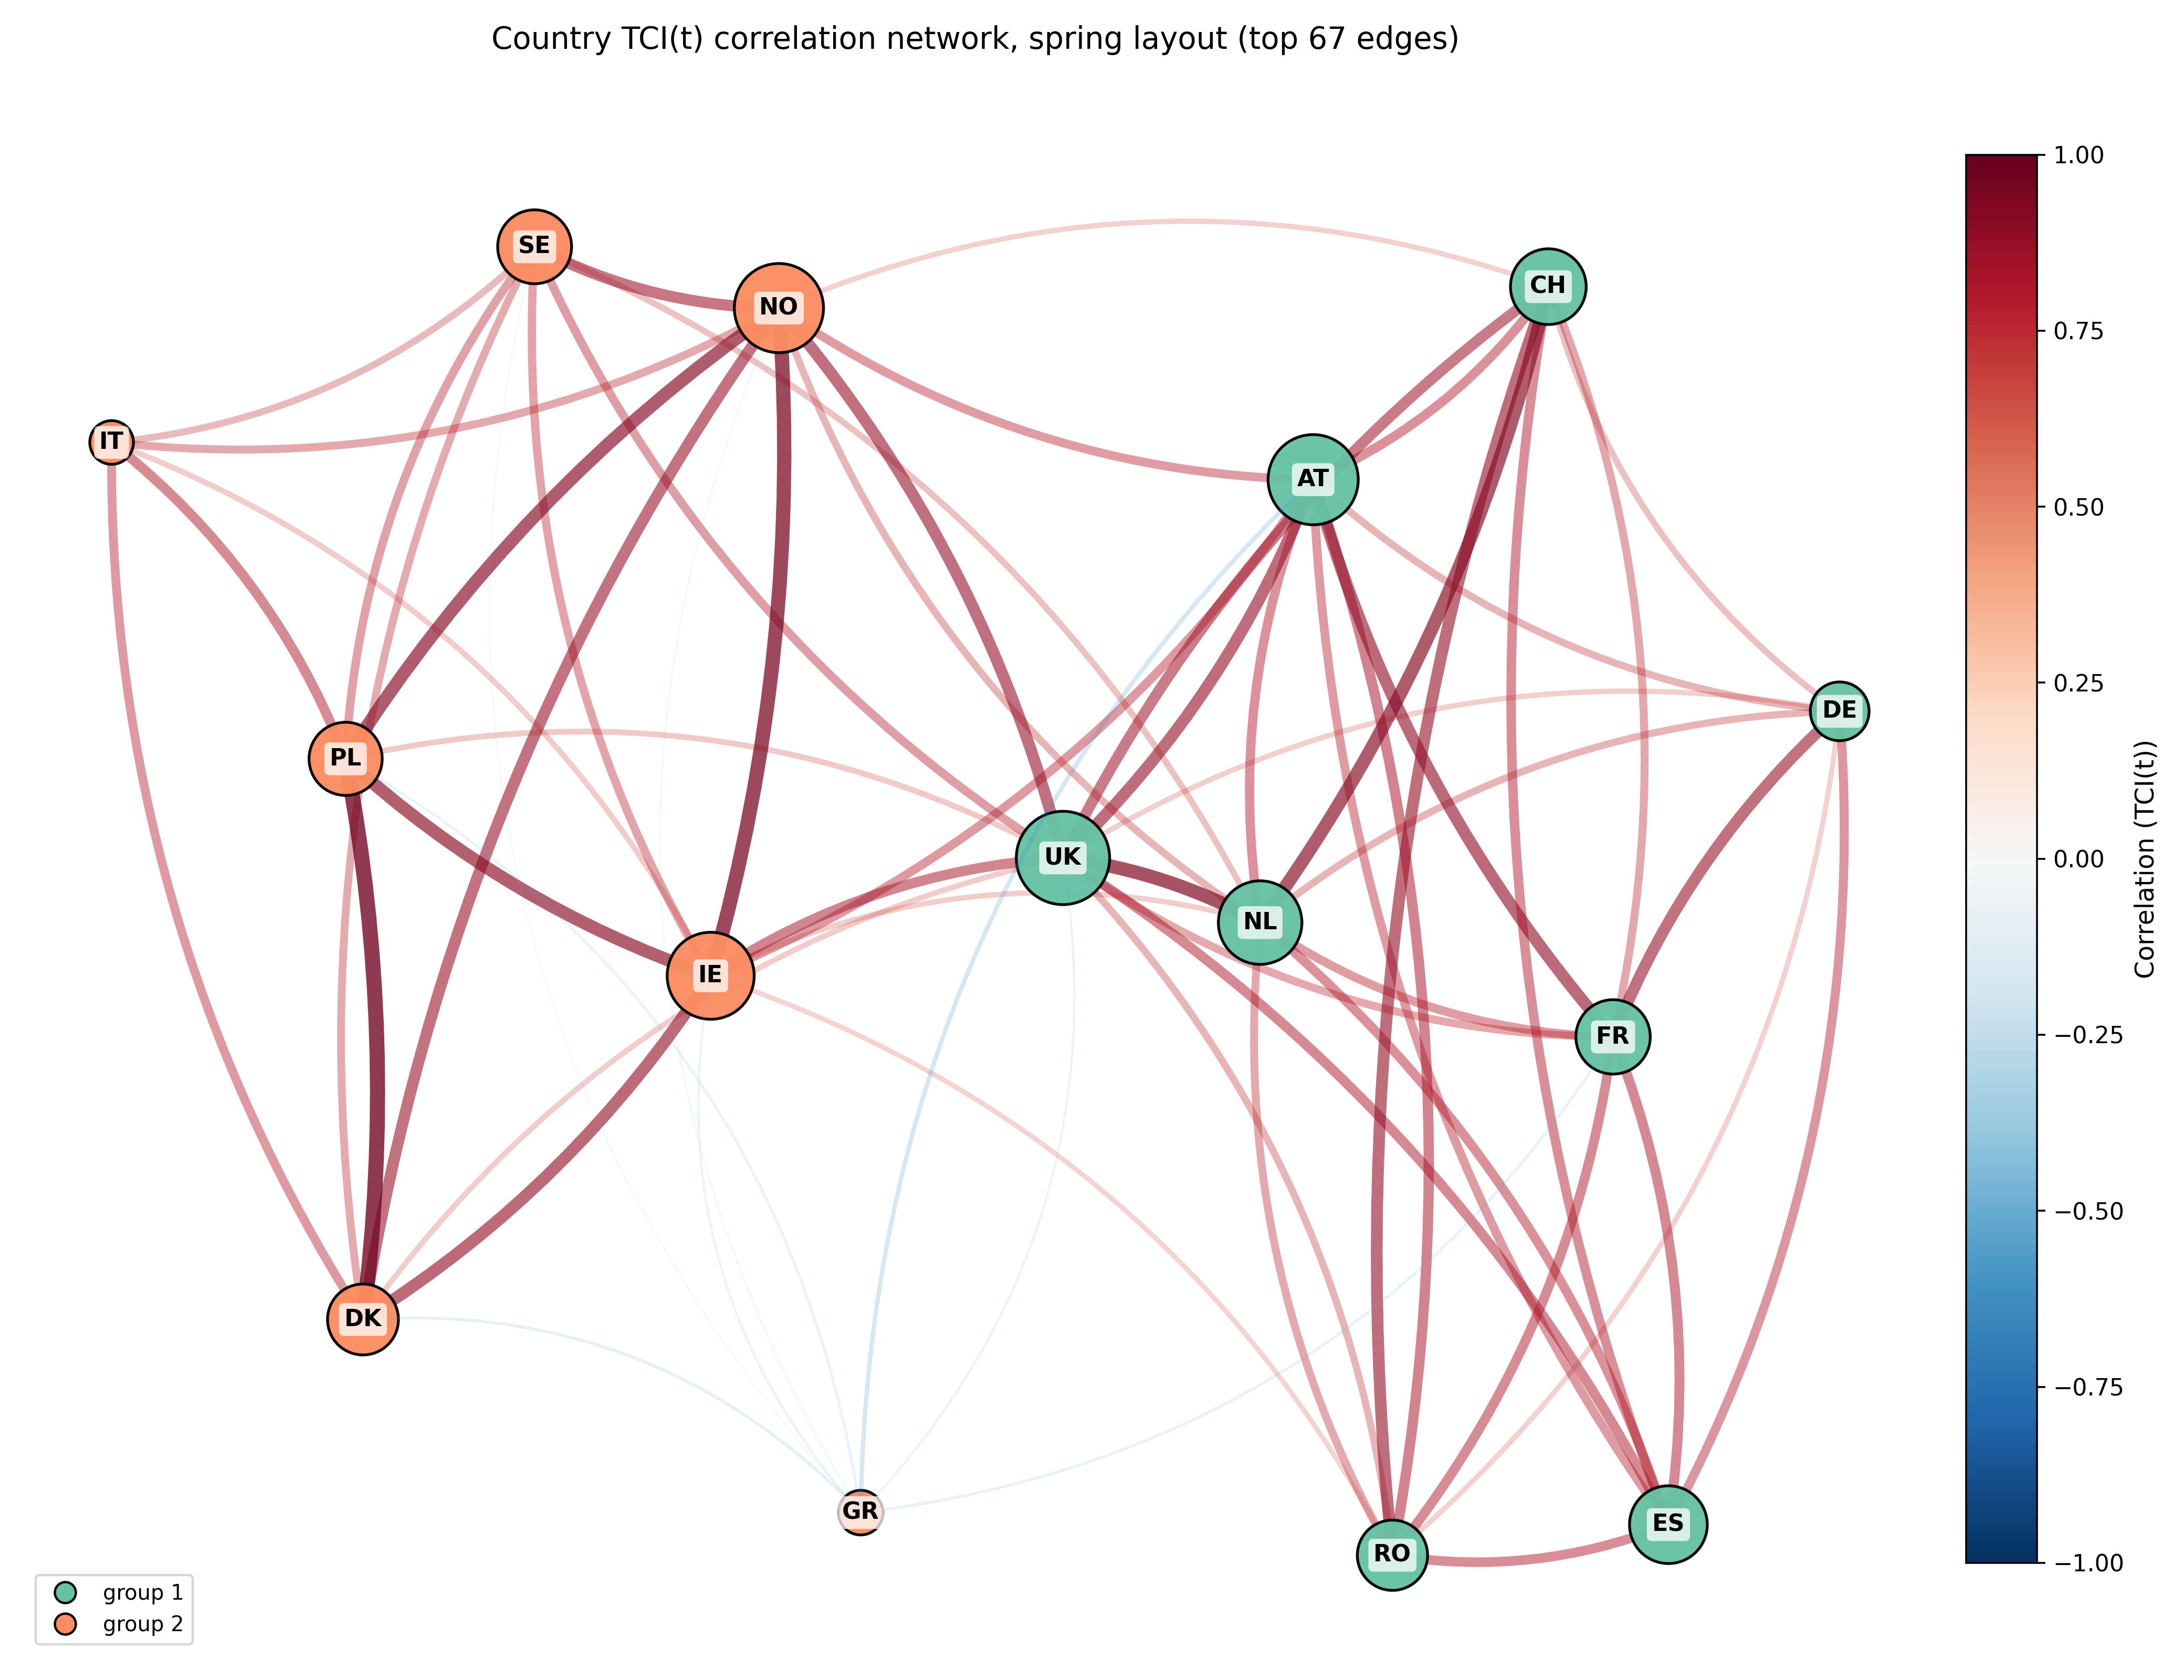
\includegraphics[width=\textwidth]{tci_country_corr_network.png}
  \caption{Country-level correlation network of banking connectedness dynamics. Each node
  represents a country and each edge the pairwise correlation between the temporal
  dynamics of the within-country Total Connectedness Index,
  $\rho_{ij} = \mathrm{Corr}(\mathrm{TCI}_i(t),\,\mathrm{TCI}_j(t))$, computed over the
  full sample period. Node positions are determined by a spring layout algorithm
  (Fruchterman--Reingold), so that countries with more similar connectedness dynamics are
  placed closer together. Edge thickness reflects the magnitude of the correlation, while
  edge colour indicates its sign: red denotes positive correlations and blue denotes
  negative correlations. Node size is proportional to each country's overall
  connectedness with the rest of the system. Node colours identify communities detected
  by the Louvain algorithm (\texttt{python-louvain}, seed $= 7$). Community assignments
  are perfectly stable across 100 random restarts (mean NMI $= 1.00$), confirming that the
  five-group structure is fully robust to algorithmic randomness.}
  \label{fig:tci_country_corr_network}
\end{figure}

Figure~\ref{fig:tci_country_corr_network} complements the country-level TCI panels by
offering a structural, network-based perspective on how banking connectedness dynamics
co-evolve across European countries. Rather than measuring direct spillovers between
individual institutions, the graph is built from the pairwise correlation matrix of the country-level TCI series
($\rho_{ij}$, as defined in the figure caption), so that each edge summarises the degree
to which two national banking systems experience similar fluctuations in domestic
connectedness over the full sample.

Several features stand out. First, the network exhibits a clear core--periphery
structure: countries such as the United Kingdom, the Netherlands, France, and Germany
occupy central positions with many strong positive edges, while countries such as Sweden,
Italy, and Greece are comparatively more isolated. This is consistent with the TCI
time-series evidence, where core Eurozone markets displayed smoother and more persistently
high connectedness paths relative to peripheral or smaller markets. Second, the Louvain
communities highlight the presence of distinct regional clusters of banking systems that
share common systemic behaviour: in particular, a group of Central and Eastern European
countries (e.g.\ PL, RO) forms a cluster more loosely connected to the Western European
core, suggesting that their domestic connectedness dynamics are driven by partially
distinct factors. Third, a small number of negative edges (blue links) indicates that
certain pairs of countries experience inversely related connectedness cycles, which is of
particular interest from a diversification standpoint.

In the next section, we exploit this information when comparing spillover-informed
portfolio tilts with allocation schemes based on correlation and MST clustering.

\paragraph{Between-country directional spillovers.}

The within-country TCI and the correlation network above characterise how domestic
connectedness \emph{co-moves} across countries, but they do not measure the direct
transmission of volatility shocks \emph{from} one national banking system \emph{to}
another. To fill this gap, we compute the average between-country directional spillover

\begin{equation}\label{eq:S_between}
  S_{c \to c',w} \;=\;
  \frac{1}{|G_c|\,|G_{c'}|}
  \sum_{i \in G_c}\sum_{j \in G_{c'}}
  \tilde{\theta}^{g}_{ij,w}(H),
\end{equation}

\noindent where $G_c$ and $G_{c'}$ denote the sets of institutions headquartered in
countries $c$ and $c'$ respectively and $\tilde{\theta}^{g}_{ij,w}(H)$ is the
GFEVD-based spillover from institution $i$ to institution $j$ at horizon $H$ in rolling
window $w$. $S_{c \to c'}$ is then averaged across all windows to obtain a single
full-sample measure.

Figure~\ref{fig:country_spillover_heatmap} displays the resulting $18 \times 18$
directional spillover matrix. The matrix is clearly asymmetric, highlighting genuine
directionality in cross-border shock transmission. Rows with uniformly high values
identify the main \emph{exporting} national systems, while columns with high values
mark the main \emph{recipients}. Large, cross-border banking systems (UK, FR, DE, ES)
tend to display the highest outgoing spillover rows, consistent with their central role
in the within-institution analysis.

\begin{figure}[htbp]
  \centering
  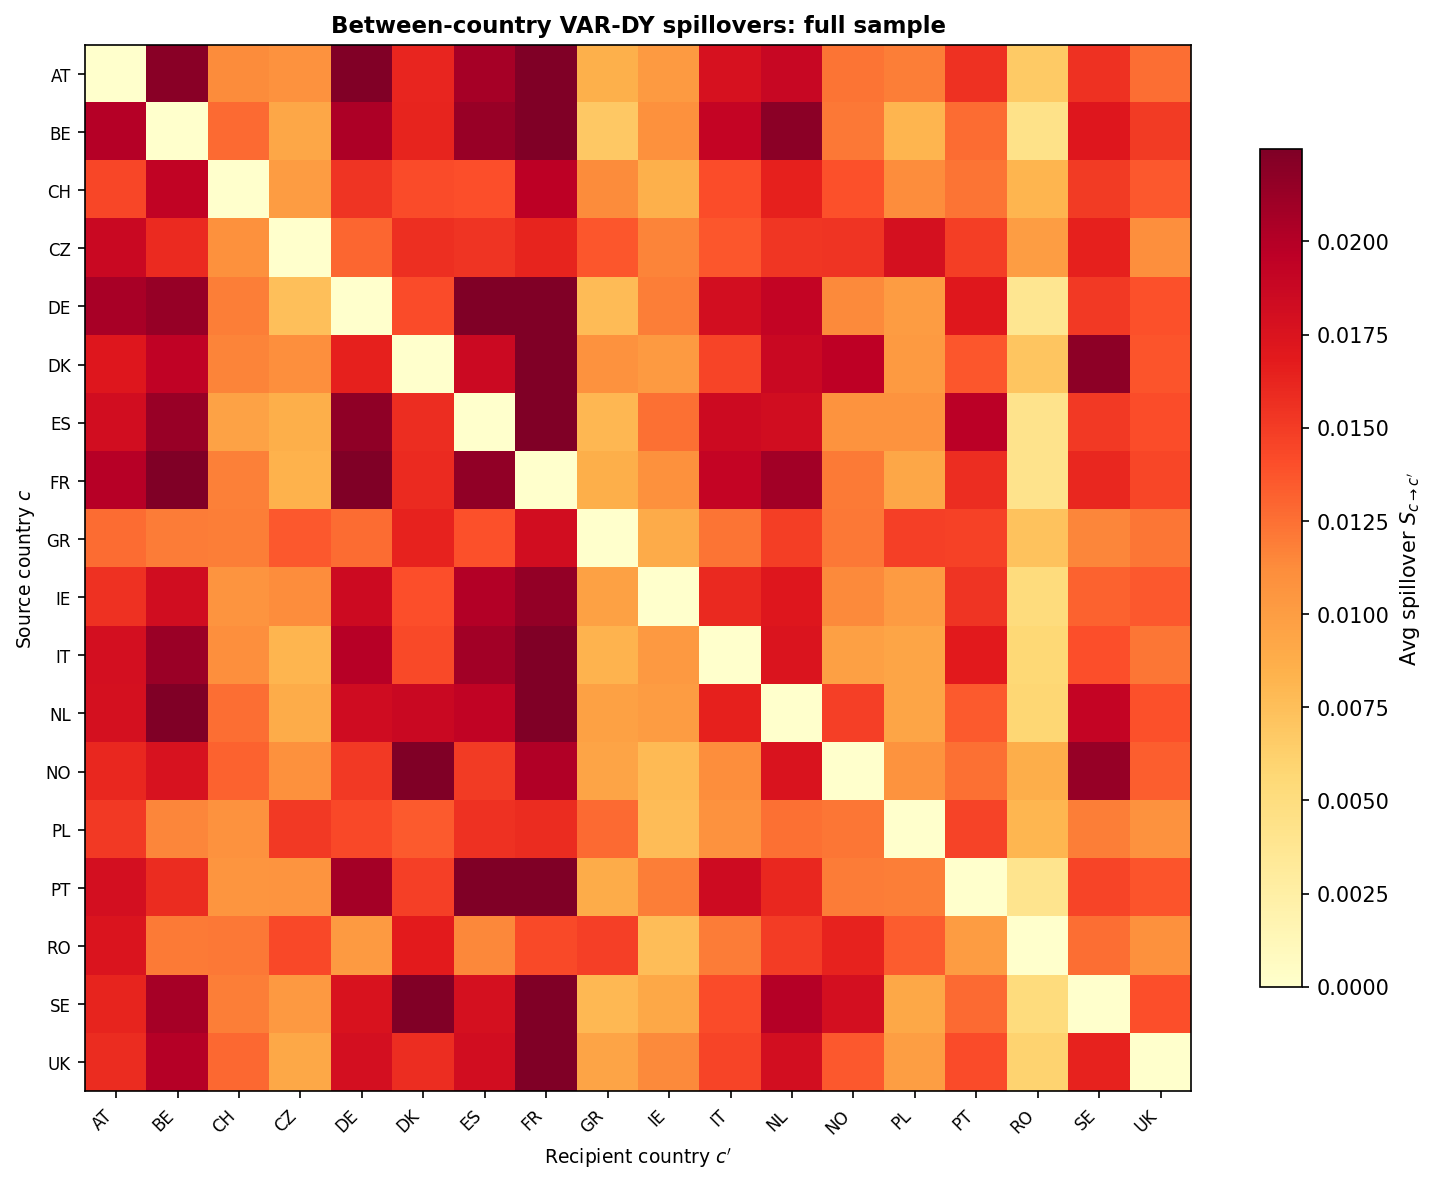
\includegraphics[width=0.85\textwidth]{country_spillover_heatmap_full.png}
  \caption{Between-country VAR--DY spillover matrix $S_{c \to c'}$ averaged over the
  full sample. Row $c$, column $c'$ gives the average fraction of forecast-error
  variance of country $c'$'s institutions explained by shocks originating in country
  $c$'s institutions. Colour scale: light = weak spillover, dark red = strong spillover.}
  \label{fig:country_spillover_heatmap}
\end{figure}

Figure~\ref{fig:country_spillover_network} translates the matrix into a directed network
in which edge colour and width encode the magnitude of $S_{c \to c'}$ (light orange to
dark red) and node colour encodes the net spillover position
$S_{c \to \cdot} - S_{\cdot \to c}$ (red = net emitter, blue = net receiver). The
figure reveals a clear hierarchy: a small group of Western European banking systems
consistently transmit more volatility than they receive, while smaller or more
domestically oriented markets occupy net-receiver positions.

\begin{figure}[htbp]
  \centering
  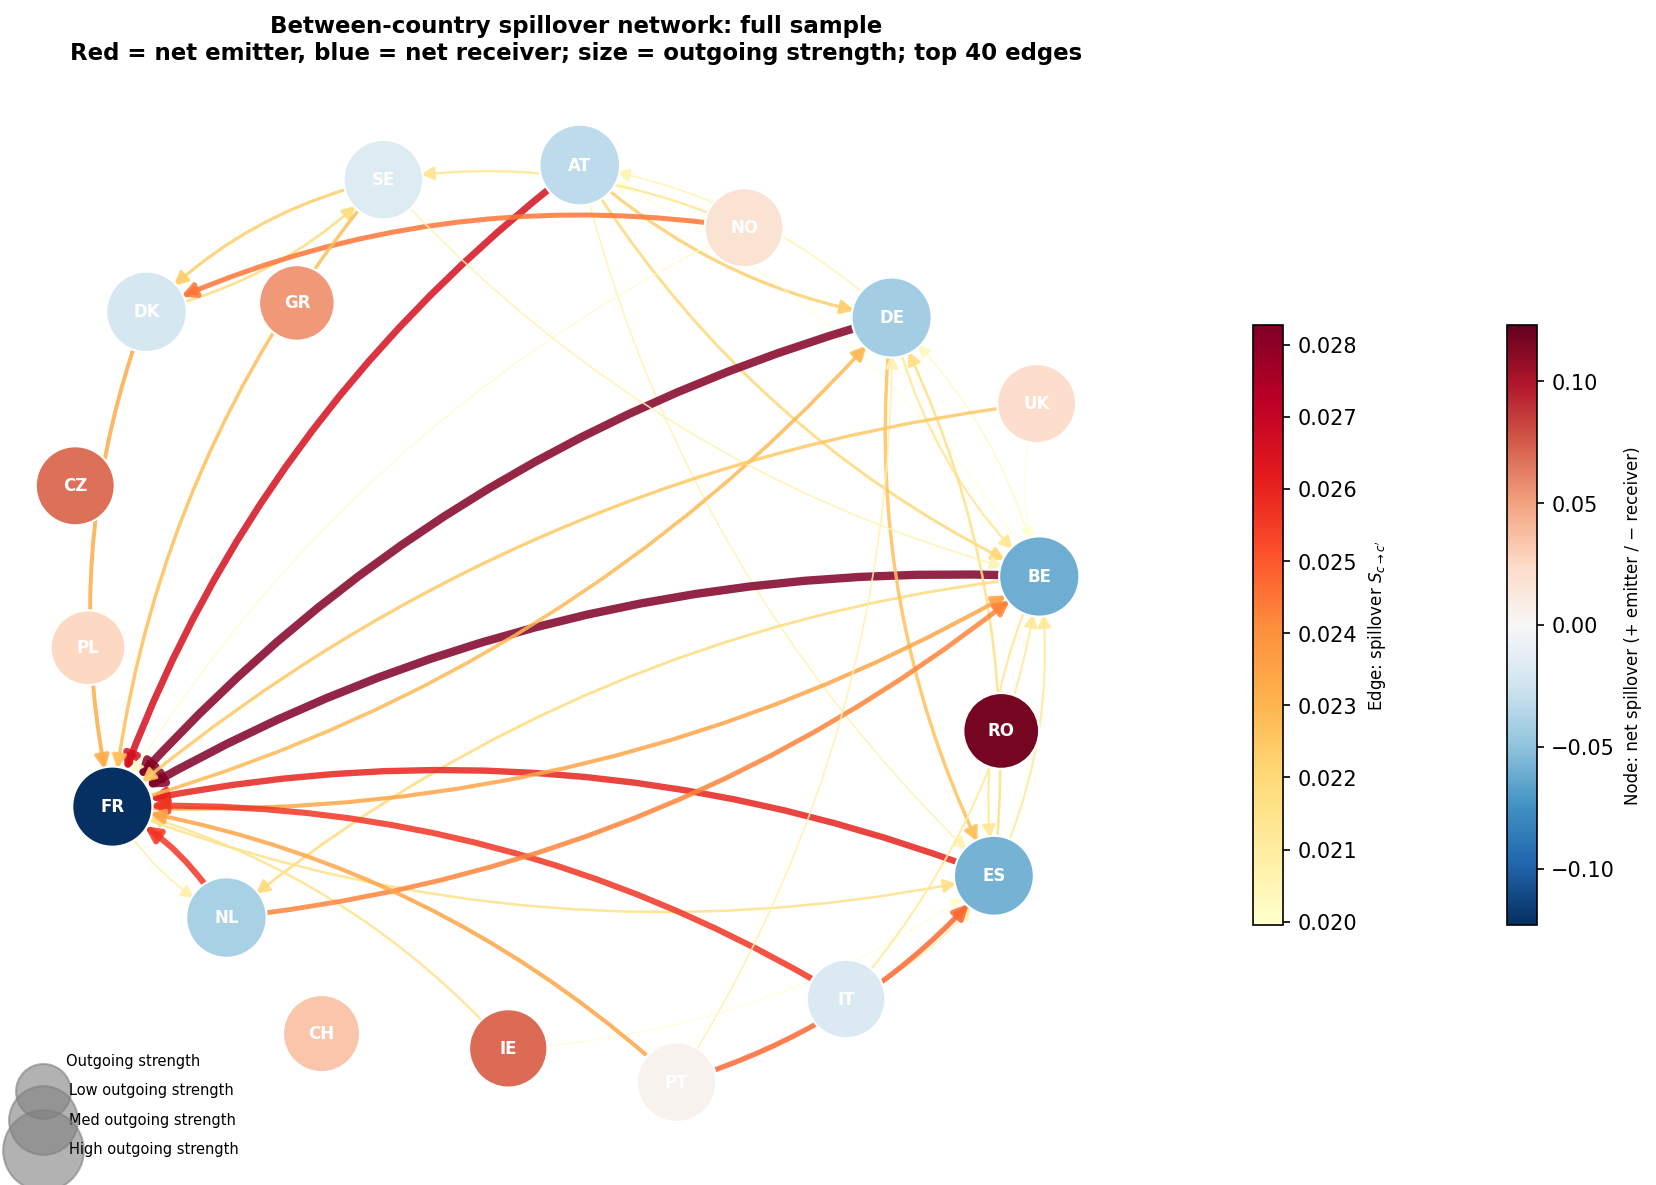
\includegraphics[width=0.85\textwidth]{country_spillover_network_full.png}
  \caption{Directed between-country VAR--DY spillover network (full sample, top 40 edges).
  Node colour: red = net spillover emitter, blue = net receiver.
  Node size: total outgoing spillover strength.
  Edge colour and width: magnitude of $S_{c \to c'}$ (light orange to dark red).}
  \label{fig:country_spillover_network}
\end{figure}
